\documentclass[10pt,letterpaper]{article}
\renewcommand\familydefault{\sfdefault}

\usepackage{amsmath}

\usepackage[T1]{fontenc} 
\usepackage[utf8x]{inputenc}
\usepackage[british]{babel}
\usepackage{graphicx}% Include figure files
\usepackage{blindtext} 

\usepackage{fancyvrb,xcolor}
\usepackage{upquote,textcomp}

%%% Margins
\oddsidemargin=-0.50cm
\textwidth=17.0cm
\topmargin=-2.54cm
\headheight=0cm
\headsep=2cm
\textheight=23.8cm


\usepackage{hyperref} % for urls


% Default fixed font does not support bold face
\DeclareFixedFont{\ttb}{T1}{txtt}{bx}{n}{8} % for bold
\DeclareFixedFont{\ttm}{T1}{txtt}{m}{n}{8}  % for normal

% Custom colors
\usepackage{color}
\definecolor{deepblue}{rgb}{0,0,0.5}
\definecolor{deepred}{rgb}{0.6,0,0}
\definecolor{deepgreen}{rgb}{0,0.5,0}
\definecolor{deepgray}{rgb}{0.5,0.5,0.5}

\usepackage{listings}

\lstdefinestyle{myCustomPythonStyle}{
	language=Python,
	basicstyle=\linespread{1}\small,
	otherkeywords={self},             % Add keywords here
	keywordstyle=\ttb\color{deepblue},
	emph={MyClass,__init__},          % Custom highlighting
	emphstyle=\ttm\color{deepred},    % Custom highlighting style
	commentstyle=\ttm\color{deepgray},
	stringstyle=\color{deepgreen},
	frame=tb,                         % Any extra options here
	showstringspaces=false,
	columns=fullflexible,
	keepspaces=true,
	literate={-}{-}1,				% To avoid problems with hyphen -
}


\usepackage{dirtree}



\makeatletter 
  \renewcommand\verbatim@font{\normalfont\ttfamily\color{blue}}
\makeatother

\parindent=0mm 			% Remove french indent
\setlength{\parskip}{0.3cm}


\title{ScientoPy - User Manual}


\begin{document}



\begin{center}

\includegraphics[scale=0.5]{./figures/scientopy_logo.eps}\\
{\LARGE \textbf{ScientoPy v 2.0.1, User Manual\\}}
\vspace*{0.5cm}

\includegraphics[scale=0.2]{./figures/escudoUnicacuaSolo.eps}\\
\vspace*{0.5cm}
Juan Pablo Ruiz Rosero\\
\texttt{jpabloruiz@unicauca.edu.co} \\
\end{center}

\tableofcontents

\newpage

\section{Installation}

1. Download the latest stable release from: \url{https://github.com/jpruiz84/ScientoPy/releases}

2. Unzip the downloaded file and run ScientoPyGui.exe

\section{Download the bibliometric dataset}
This section describes how to download the proper dataset from Scopus and WoS. Define a search criteria that will be used for Scopus and WoS. For this guide and for the example dataset we are using: "Internet of thing"  AND  "Gateway" 

\subsection{Download the dataset from Scopus}
\begin{enumerate}
\item Make your search with the defined search criteria for Article title, Abstract, Keywords. 
\item Select all the results and click on Export:
	\begin{center}
		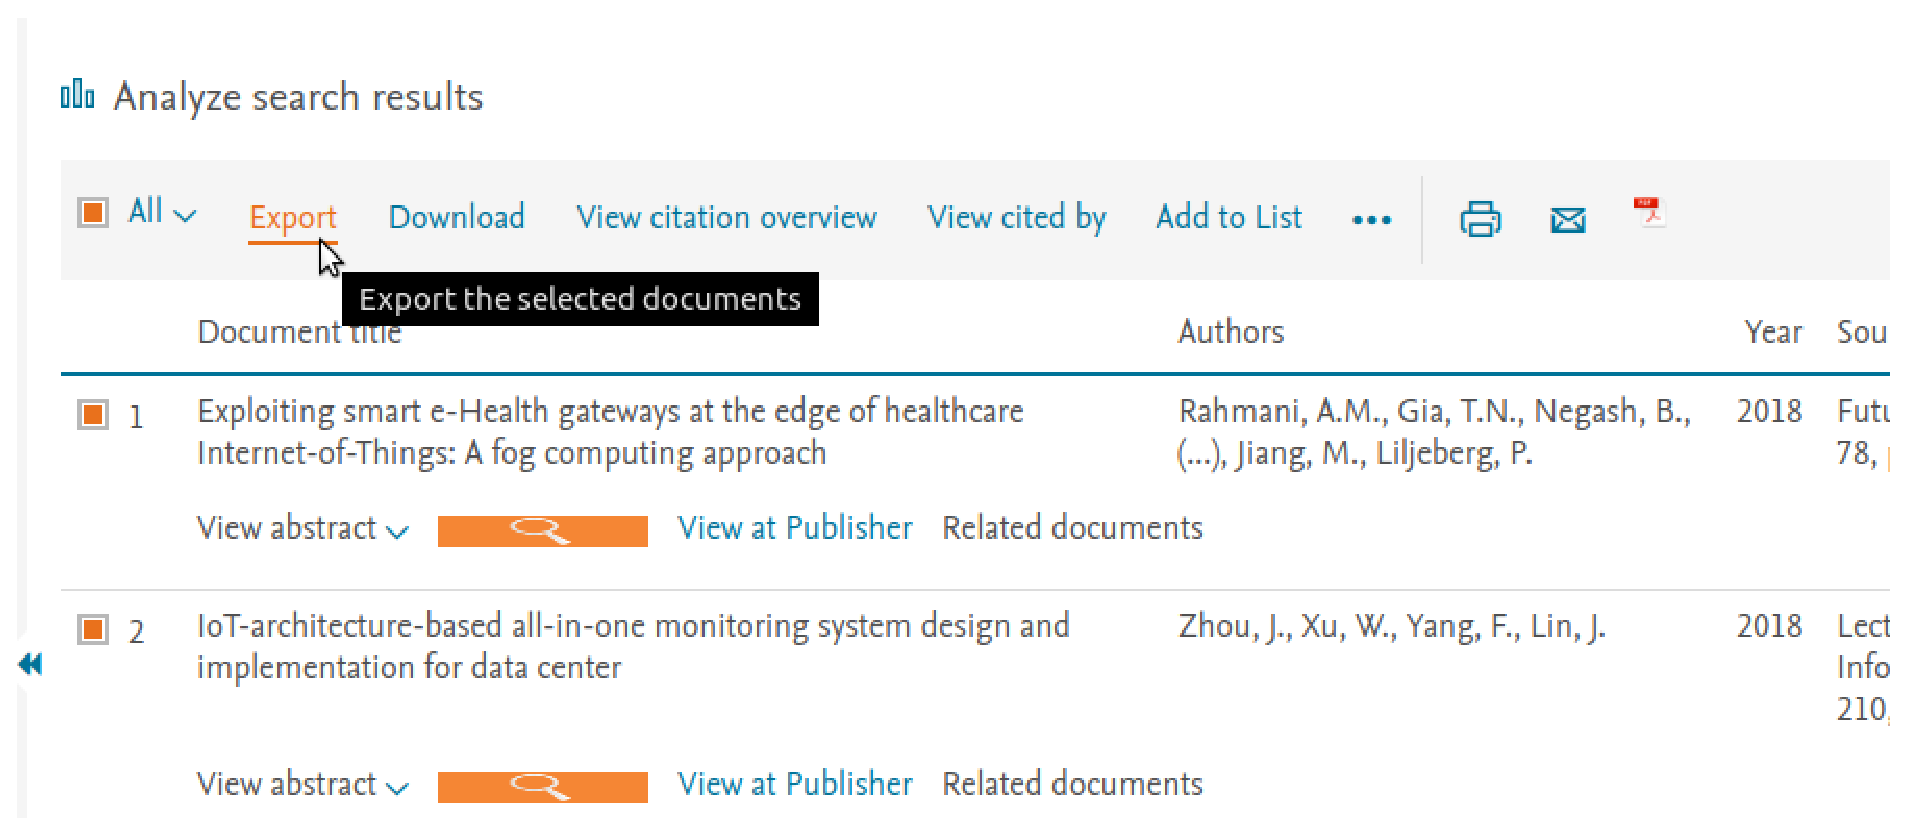
\includegraphics[scale=0.33]{./figures/scopus1.eps}
	\end{center}

\item Select as method of export \textbf{CSV (Excel)}, and select the Customize export \textbf{Citation information, Bibliographical information, Abstract and Keywords}, then click on Export: 
	\begin{center}
		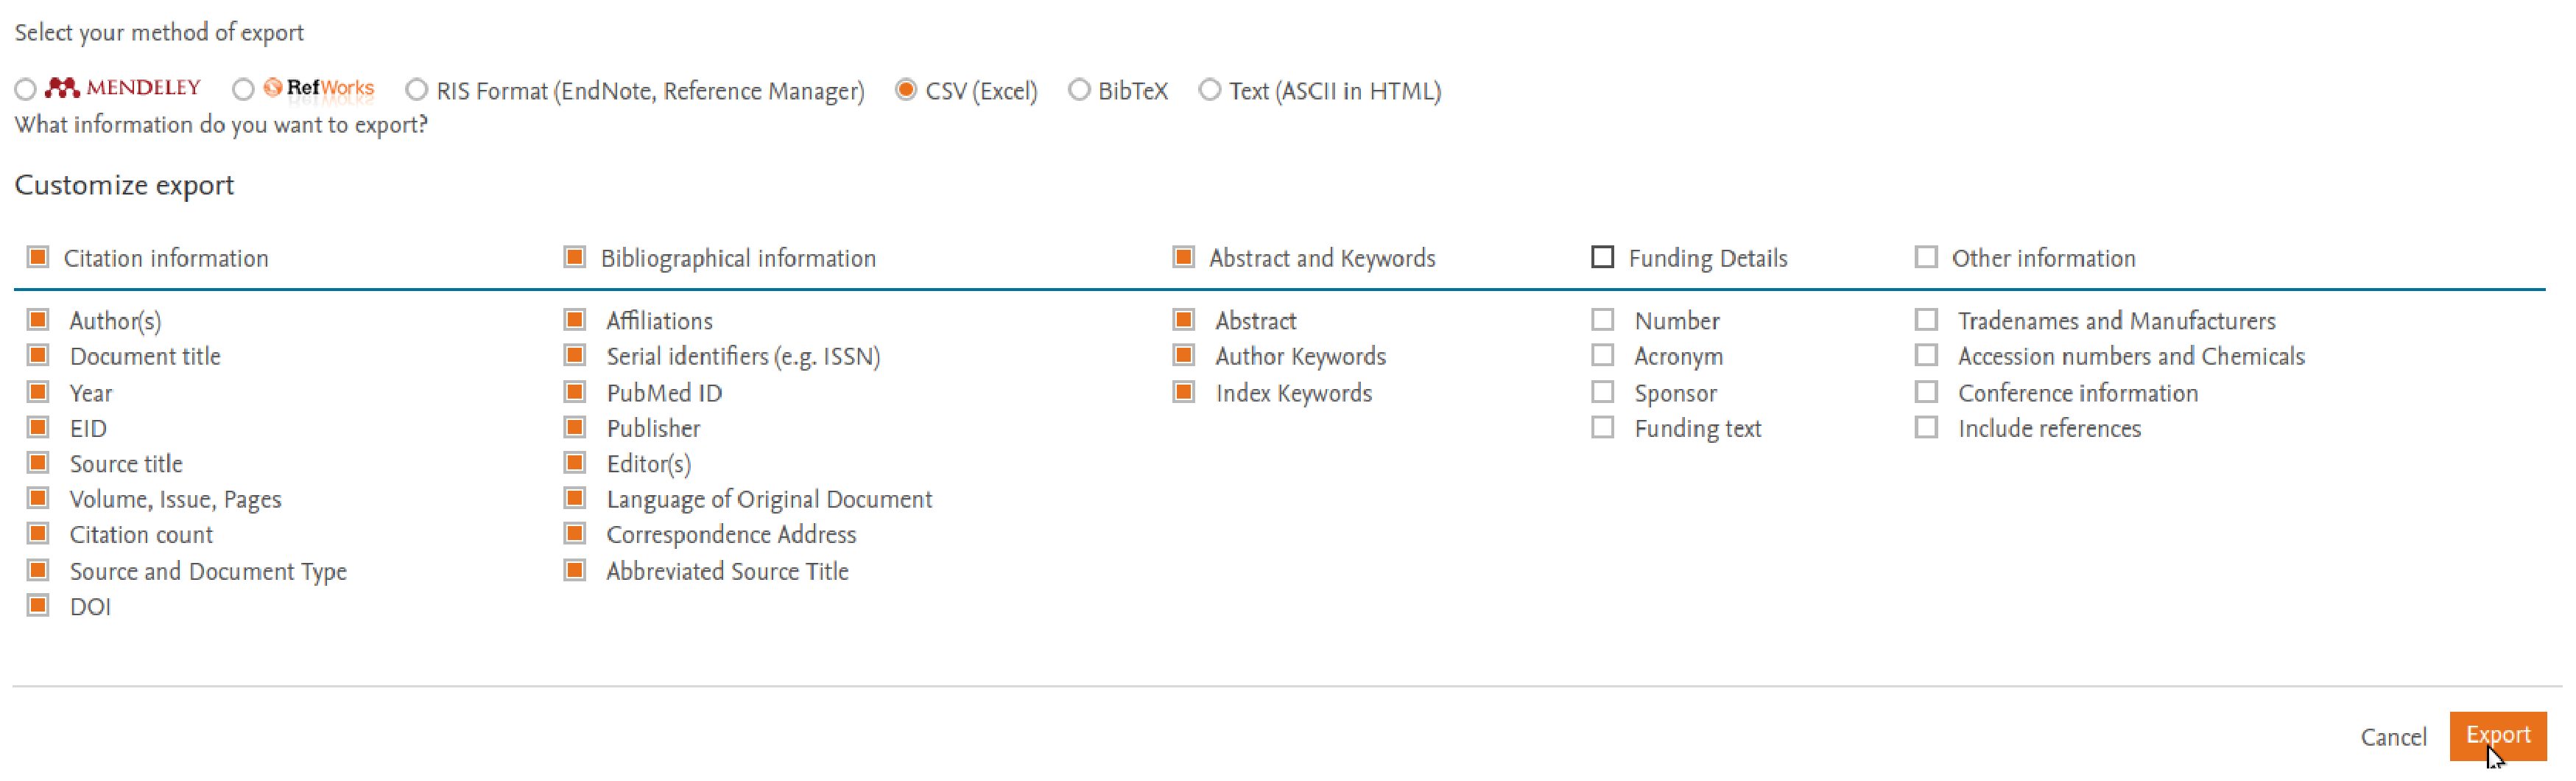
\includegraphics[scale=0.3]{./figures/scopus2.eps}
	\end{center}

\item Save the file on the folder \verb|/ScientoPy/dataIn|
\end{enumerate}


\subsection{Download the dataset from WoS}
\begin{enumerate}
\item Make your search with the defined search criteria for Topic. 
\item Select \textbf{Save in Other File Formats}
	\begin{center}
		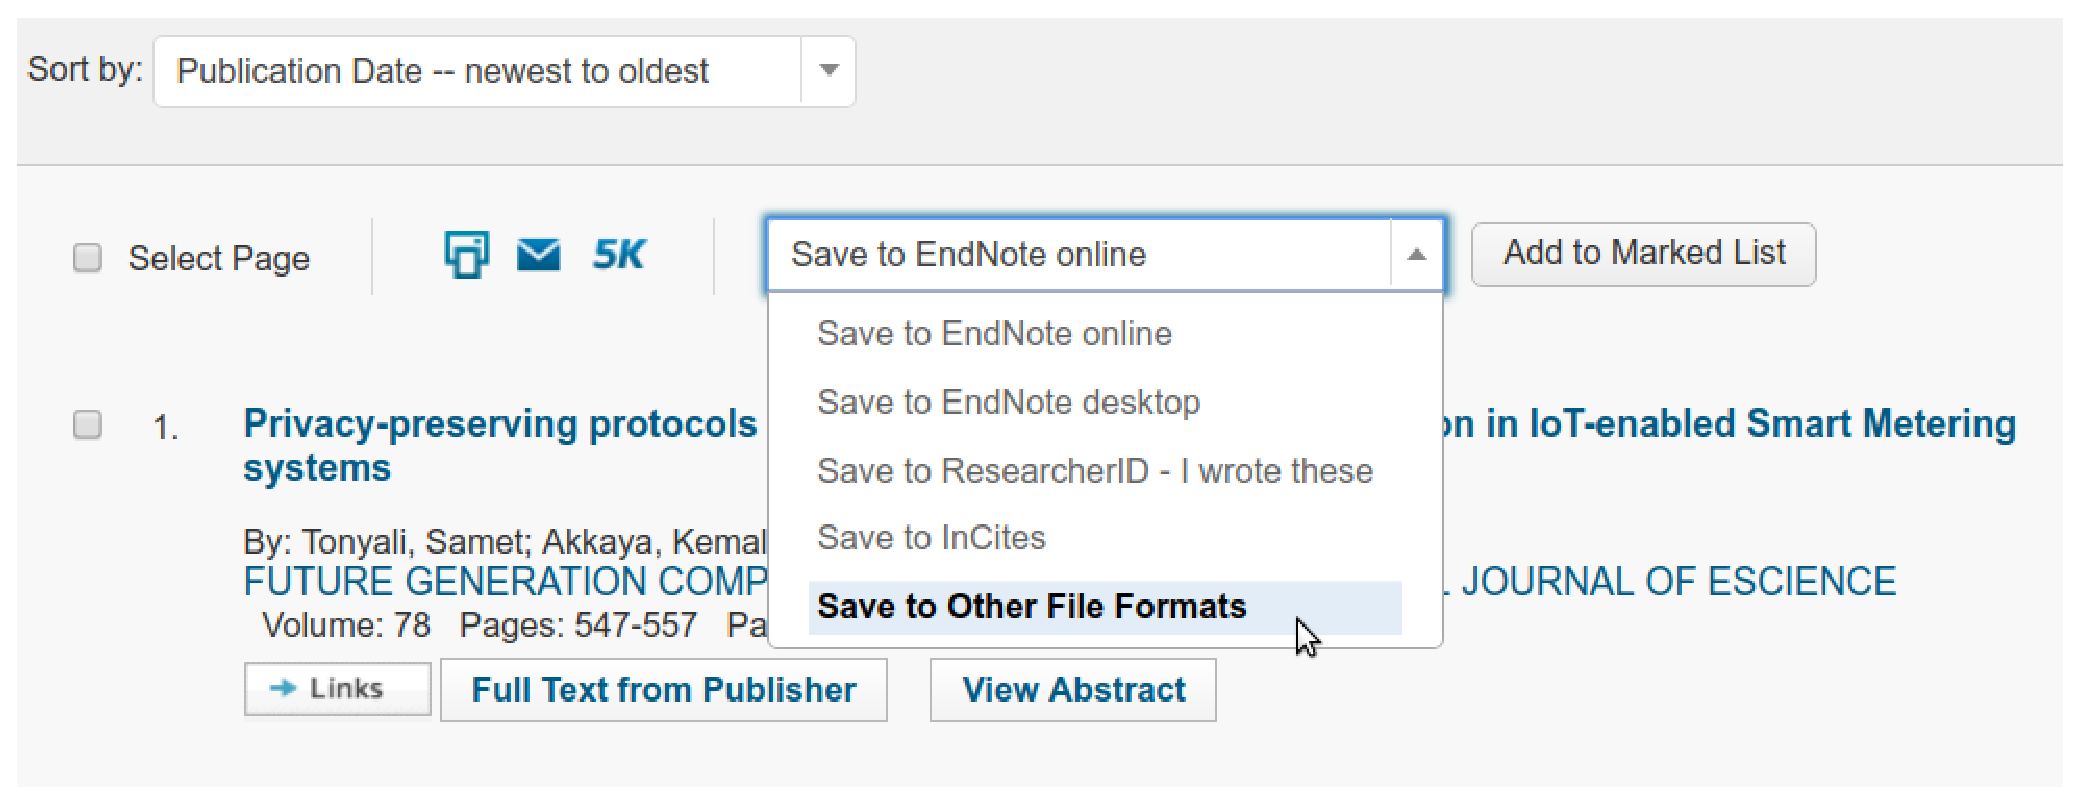
\includegraphics[scale=0.33]{./figures/wos1.eps}
	\end{center}

\item Select the number of records to download, on Record Contented select \textbf{Full Record and Cited References}, on File Format select \textbf{Tab-delimited (Win, UTF-8)}, and click on Send.
	\begin{center}
		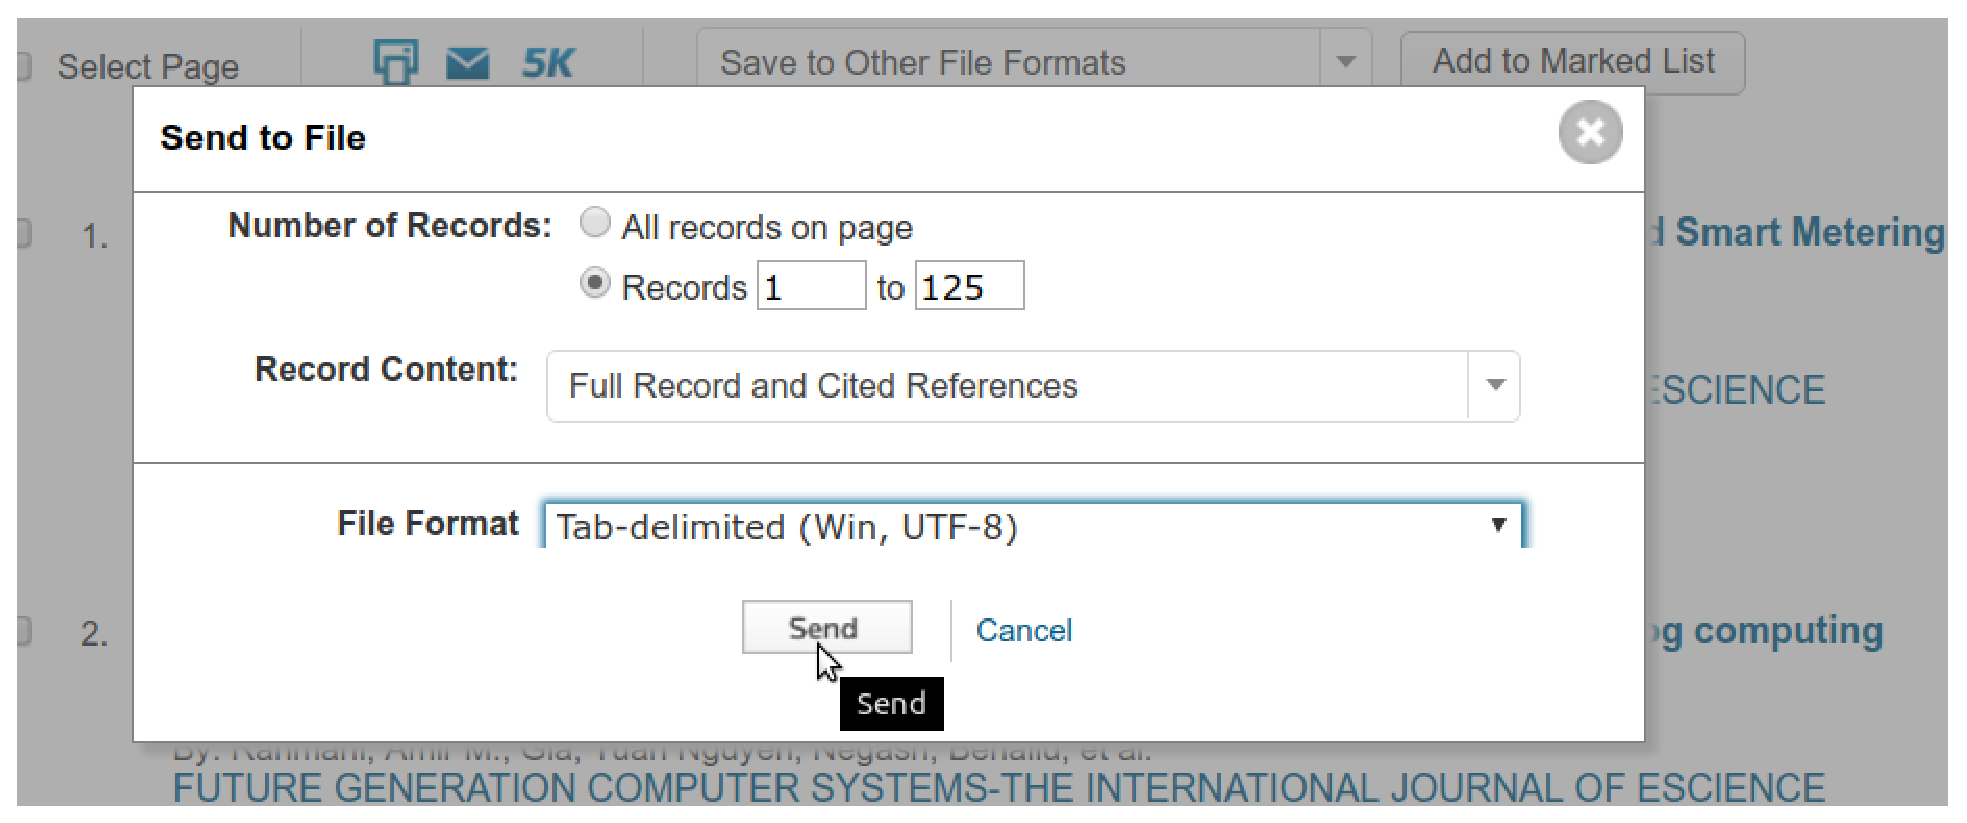
\includegraphics[scale=0.33]{./figures/wos2.eps}
	\end{center}

\item Save the file on the folder \verb|/ScientoPy/dataIn|
\end{enumerate}


\section{Preprocessing}

First we need to preprocess the downloaded dataset. This preprocess merge all the downloaded files from the dataset folder to a single file. Also, this process remove the duplicated files. To preprocess the example dataset ("Bluetooth low energy"  downloaded in March 21, 2019, located in dataInExample) open ScientoPyGui.exe and follow the next steps: 

\begin{center}
	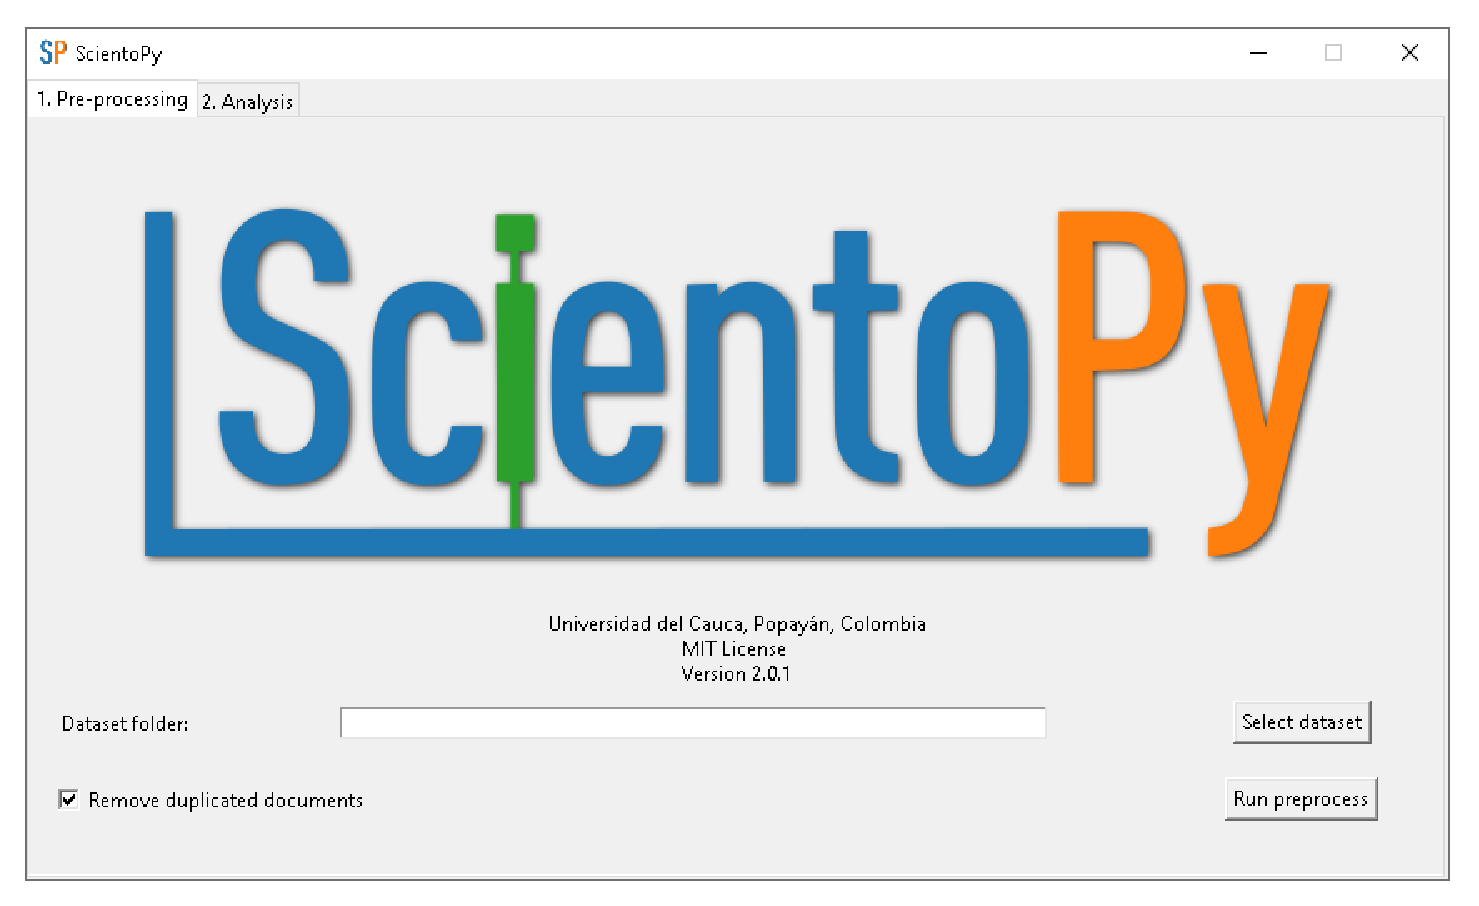
\includegraphics[width=0.75\textwidth]{./figures/win_preprocess.eps}
\end{center}

\begin{enumerate}
\item Click in \verb|Select dataset| button, and select the folder that contains the downloaded dataset. For the case of run the example dataset, select the folder \textit{dataInExample} inside ScientoPy unziped folder. 
\item Click in \verb|Run preprocess| button. This will start the preprocess. You can check the preprocess status and progress in the console output as shown in the following picture
\item After the preprocess is finished, the preprocess brief table will show up as the \textit{Output graph}. 
\end{enumerate}

\begin{center}
	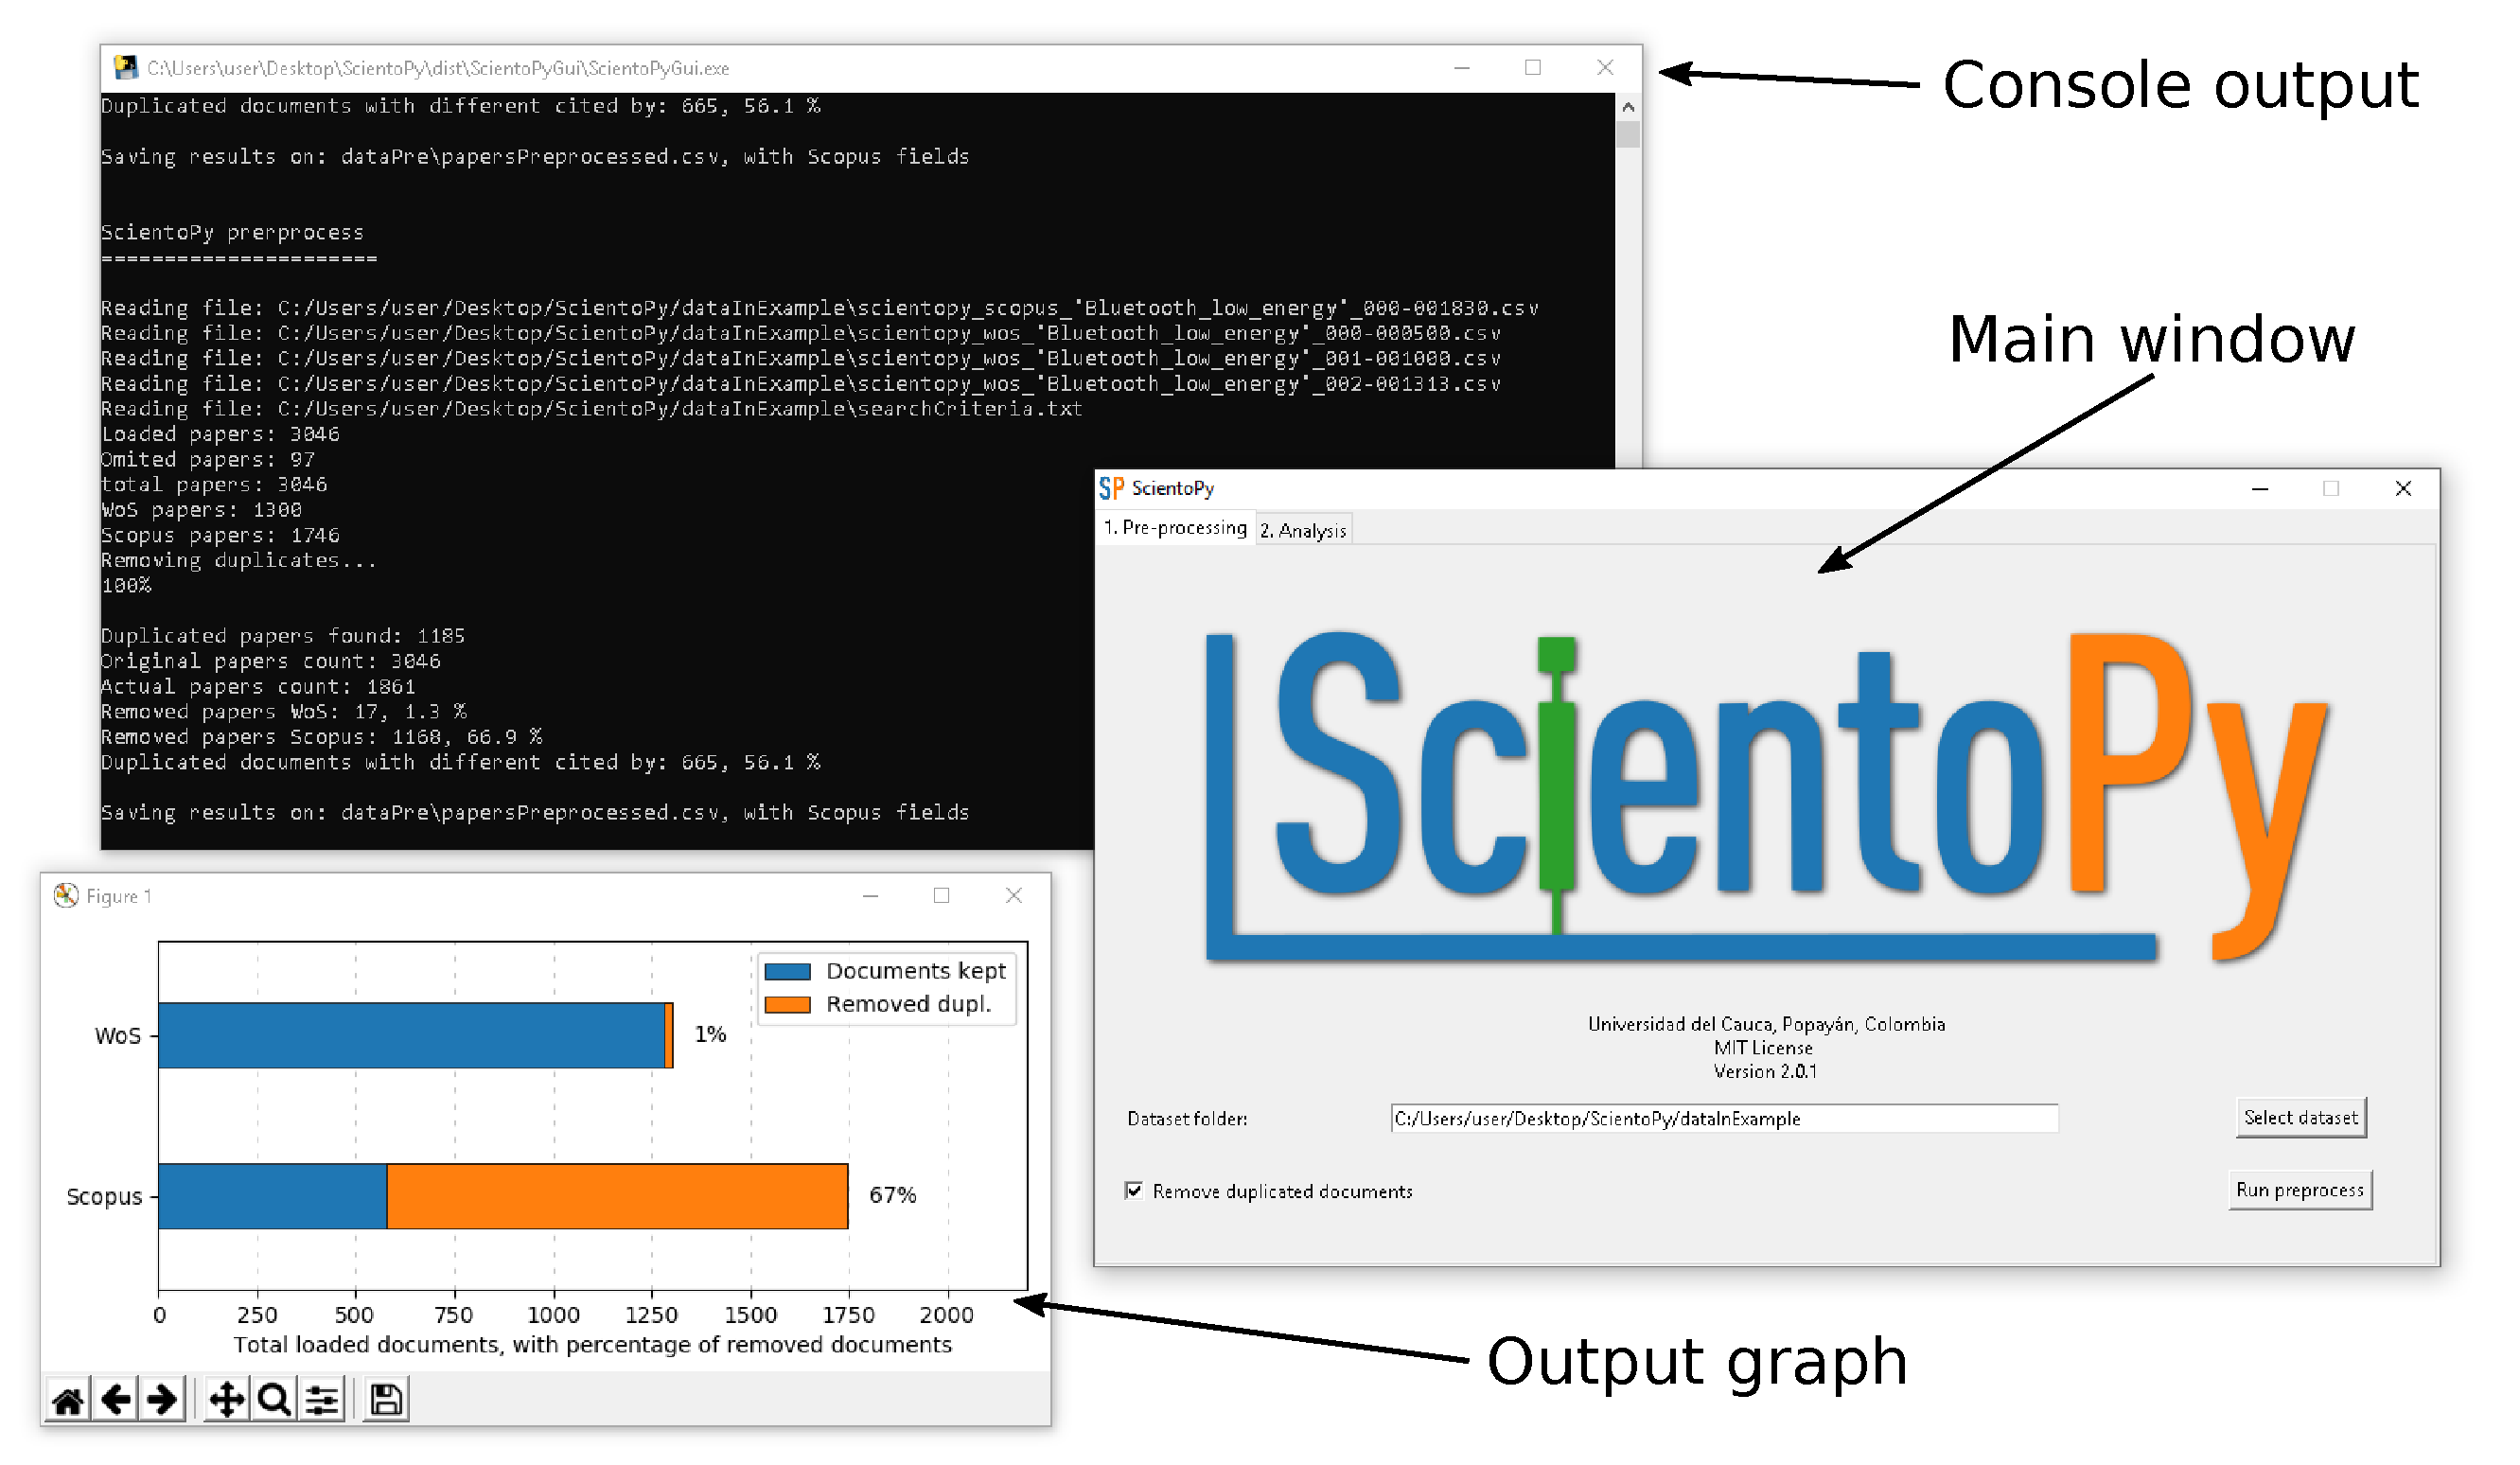
\includegraphics[width=0.9\textwidth]{./figures/win_preprocess2.eps}
\end{center}

Then, select the \verb|2. Analysis| tab, and click in \verb|Open preprocess brief| button. This will open the preprocess CSV file in Excel, as show in the following figure.

\begin{center}
	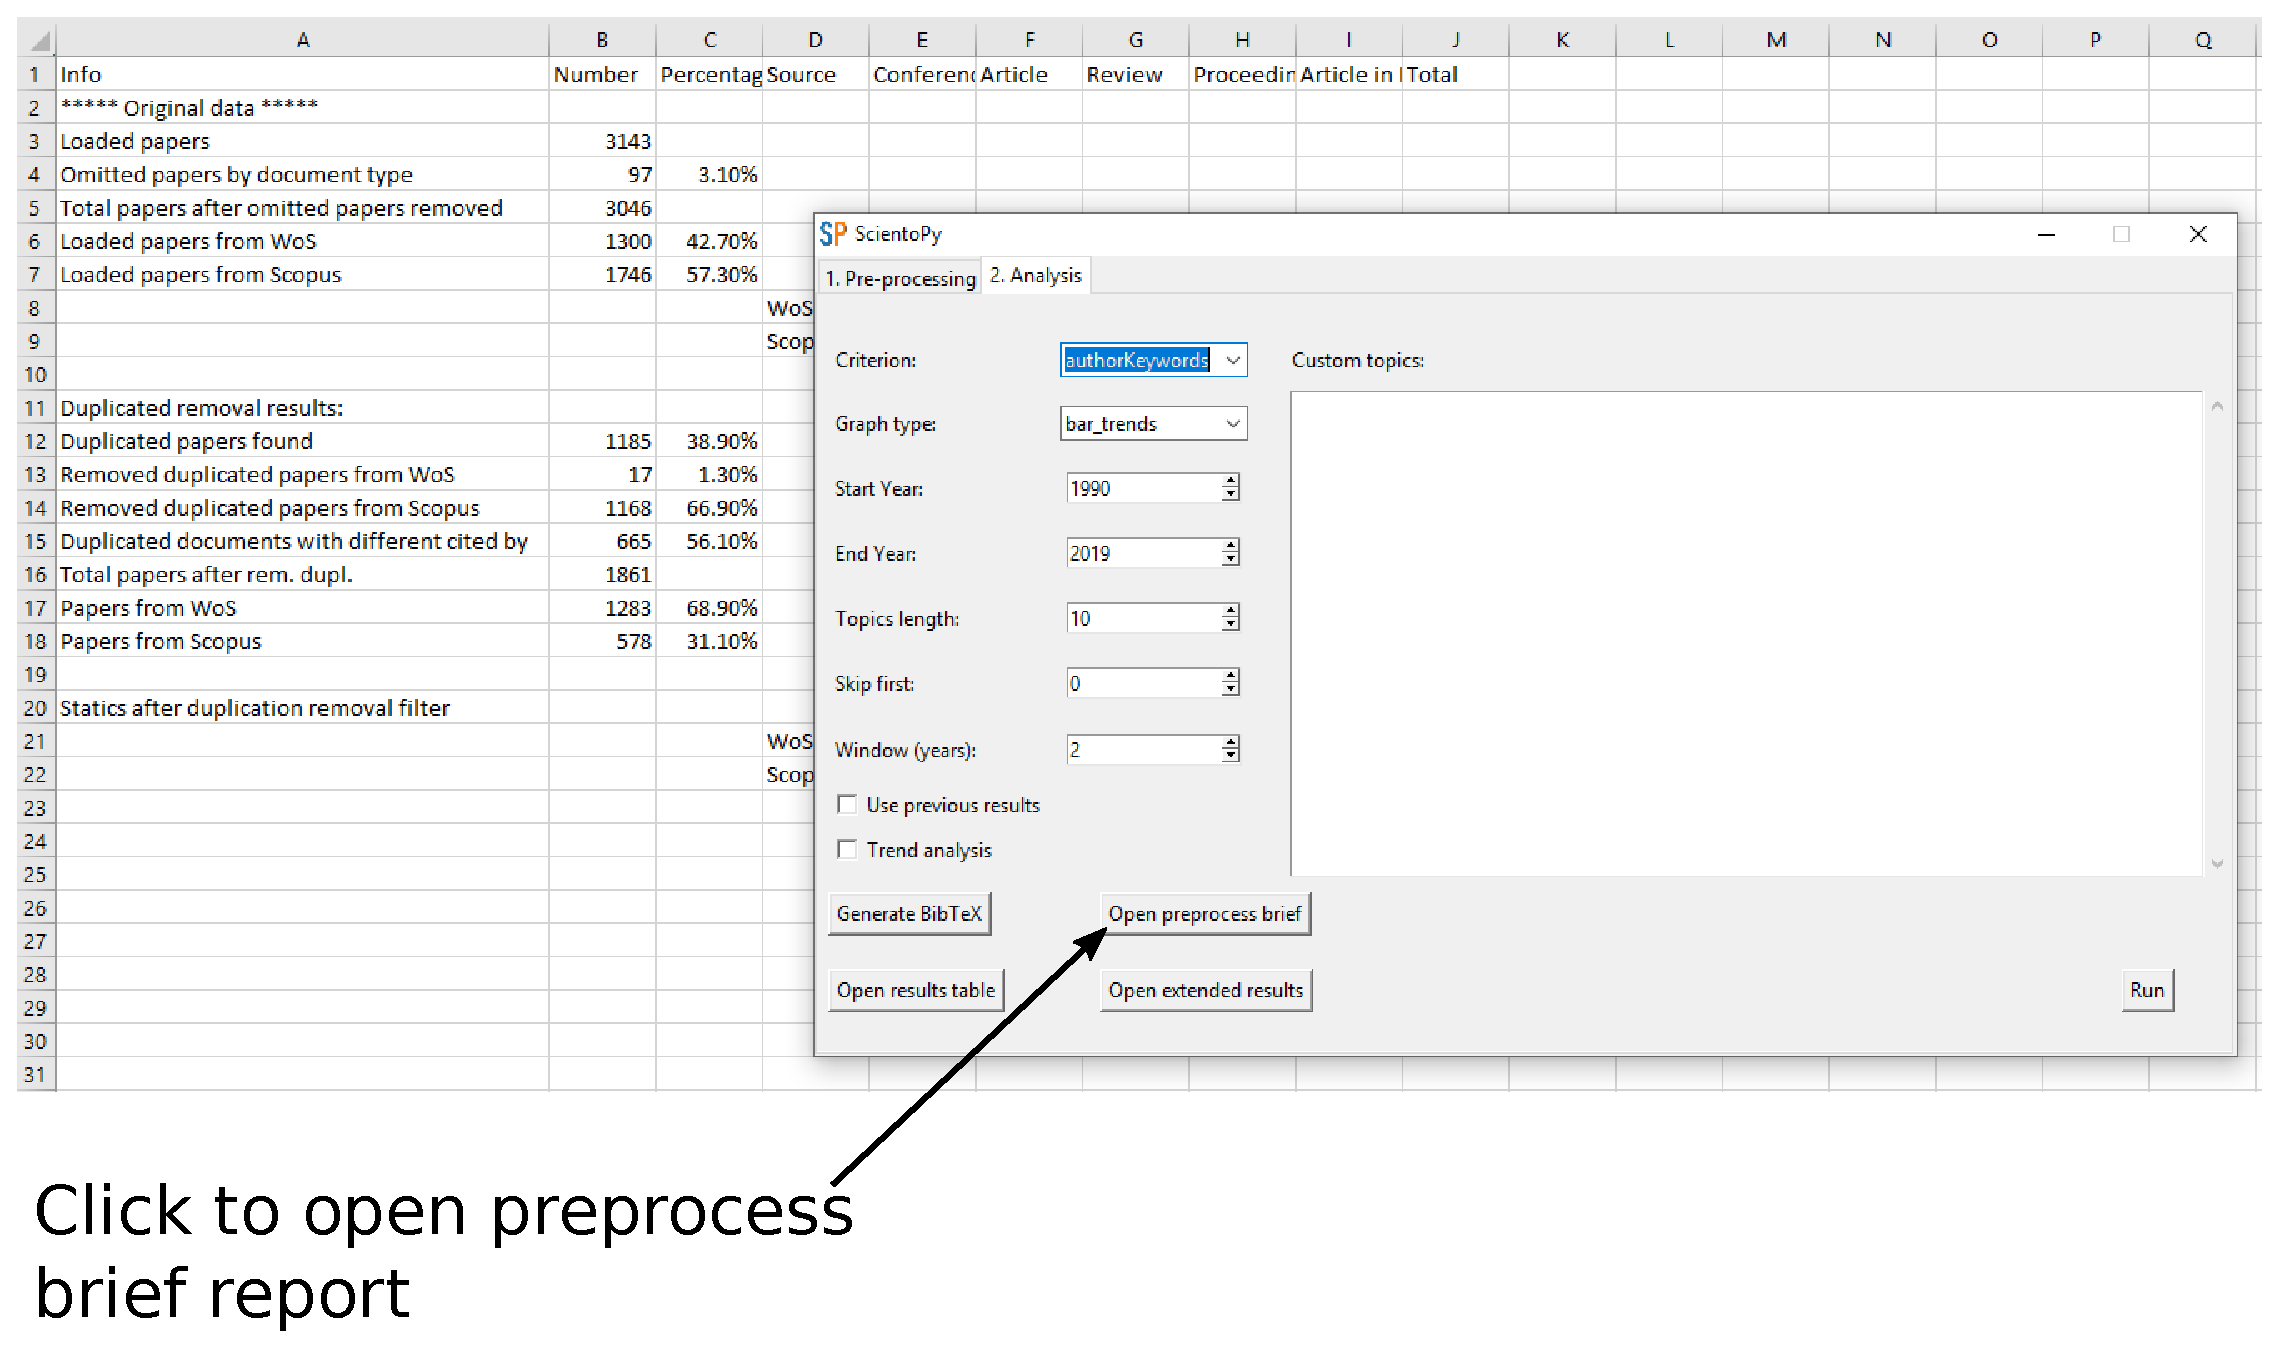
\includegraphics[width=0.8\textwidth]{./figures/win_preprocess3.eps}
\end{center}


As result, inside the folder \verb|ScientoPy/dataPre| you will find the following files: 
\begin{itemize}
\item \textbf{papersPreprocessed.tsv:} this file contains the information of all papers after the pre-process. This file will be used by the others scripts as the input data. 
\item \textbf{PreprocessedBrief.tsv:} this file briefs the pre-process statics results, such as duplicated papers removed, types of documents, and others. 
\end{itemize}


\section{Analysis page}

The analysis page let us to perform the scientometric analysis operations. To access to this page, click in the \verb|2. Analysis| tab. Then, you will see the following information described below:

\begin{center}
	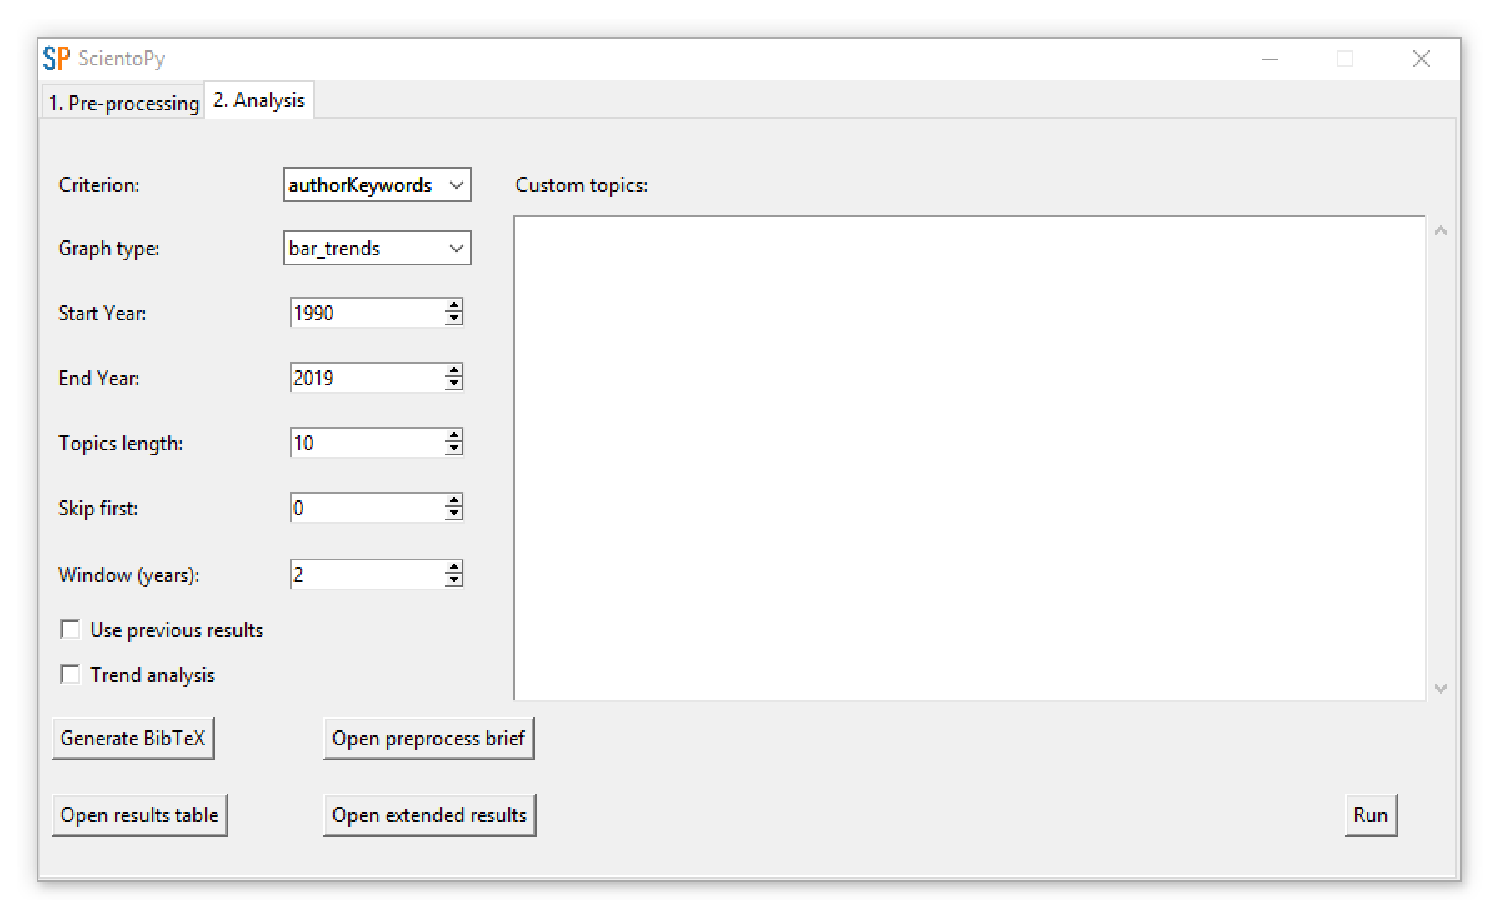
\includegraphics[width=0.8\textwidth]{./figures/win_analysis1.eps}
\end{center}

\begin{itemize}
\item \textbf{Criterion:} let the user to select the search criterion, such as author keywords, or author names. 
\item \textbf{Graph type:} define the type of the output graph.
\item \textbf{Start year:} limit the start year for the analysis and graphs.
\item \textbf{End year:} limit the end year for the analysis and graphs.
\item \textbf{Topics length:} number of top topics to find in the selected criterion.
\item \textbf{Skip first:} number of first top topics to skip during the analysis.
\item \textbf{Window (years):} window width in years for growth indicators.
\item \textbf{Use previous results:} run the analysis based on the previous results.
\item \textbf{Trend analysis:} get the top trending topics, with the highest average growth rate.
\item \textbf{Custom topics:} to enter custom topics for the analysis instead of the top topics.
\end{itemize}


The ScientoPy criterion are described on Table \ref{table_criterion}:

\begin{table}[h]
	\centering
	\caption{ScientoPy criterion description}
	\label{table_criterion}
	
	\renewcommand{\arraystretch}{1.5}
	\begin{tabular}{p{3.5cm} p{10cm}}
	\hline\noalign{\smallskip}
	Criteron       & Description                             \\
	\noalign{\smallskip}\hline\noalign{\smallskip}                                                                         
	\textbf{author}         & Authors last name and first name initial                                                                       \\
	\textbf{sourceTitle}    & Publication or journal name                                                                                    \\
	\textbf{subject}        & Research areas, only from WoS documents                                                                        \\
	\textbf{authorKeywords} & Author keywords                                                                                                \\
	\textbf{indexKeywords}  & Keywords generated by the index, from WoS \textit\{Keyword Plus\}, and from Scopus \textit\{Indexed keywords\} \\
	\textbf{bothKeywords}   & AuthorKeywords and indexKeywords are used for this search                                                      \\
	\textbf{abstract}       & Document abstract, for use with pre-defined topics and asterisk wildcard\\
	\textbf{documentType}   & Type of document                                                                                               \\
	\textbf{dataBase}       & Database where the document was extracted (WoS or Scopus)                                                      \\
	\textbf{country}        & Country extracted from authors affiliations                                                                    \\
	\textbf{institution}    & Institution extracted from authors affiliations                                                                \\
	\textbf{institutionWithCountry}    & Institution with country extracted from authors affiliations                                        \\
	\noalign{\smallskip}\hline
	\end{tabular}
	
\end{table}

\subsection{Extract top topics}

To find the top 10 author keywords, kept the default fileds in the analysis tab and push the \verb|Run| button (as shown in the following figure). This will generate a list with the top 10 topics on the selected criterion (in this case authorKeywords), with the number of documents per topic. Also, this script show the bar graph with the percentage of documents in the last years, and saves the quantitative results on the folder \verb|ScientoPy/results|. 

\begin{center}
	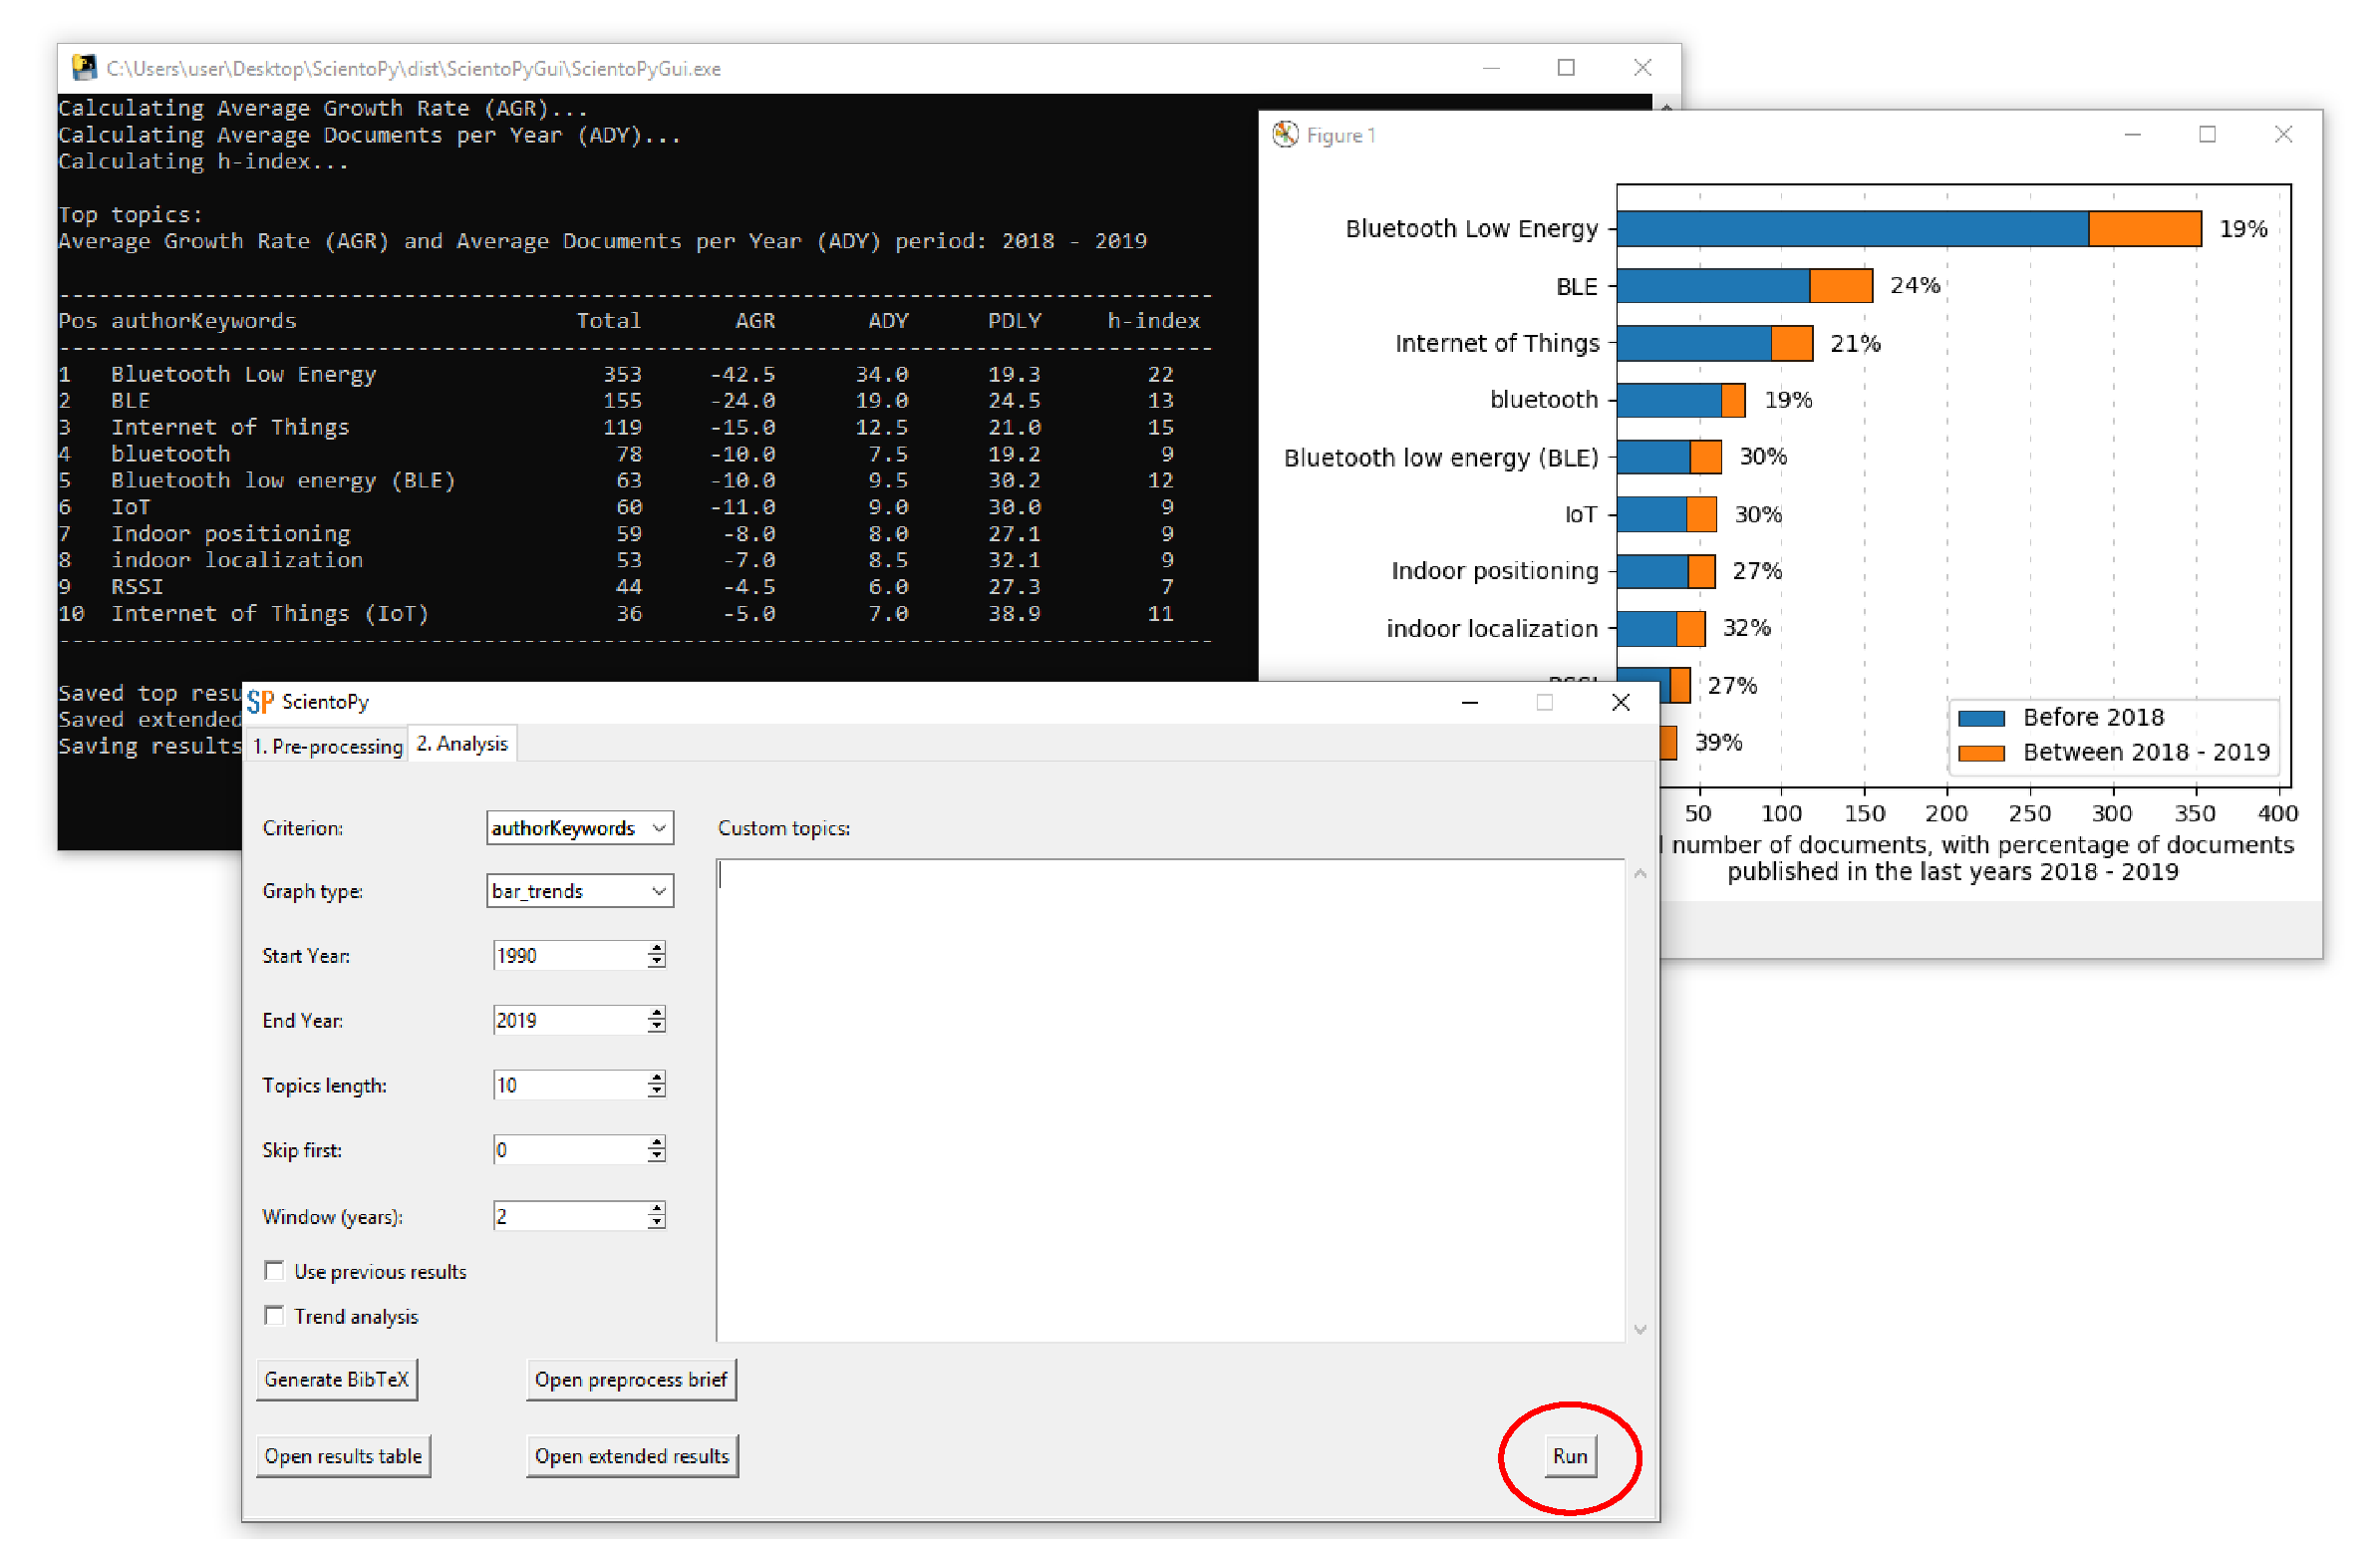
\includegraphics[width=0.8\textwidth]{./figures/win_analysis2.eps}
\end{center}

Also, the list of the top author keywords is printed in the \textit{Output console}. In the same way, you can push the \verb|Open results table| to see the quantitative results in a CSV file, or click in \verb|Open extended results| to see the CSV file with the papers related to each author keyword. 

\subsection{Analyze custom topics inside a criterion}

If you want to make an analysis of custom topics, such as the two selected countries papers evolution, you can write these in the \verb|Custom topics| text box, as shown in the following figure:

\begin{center}
	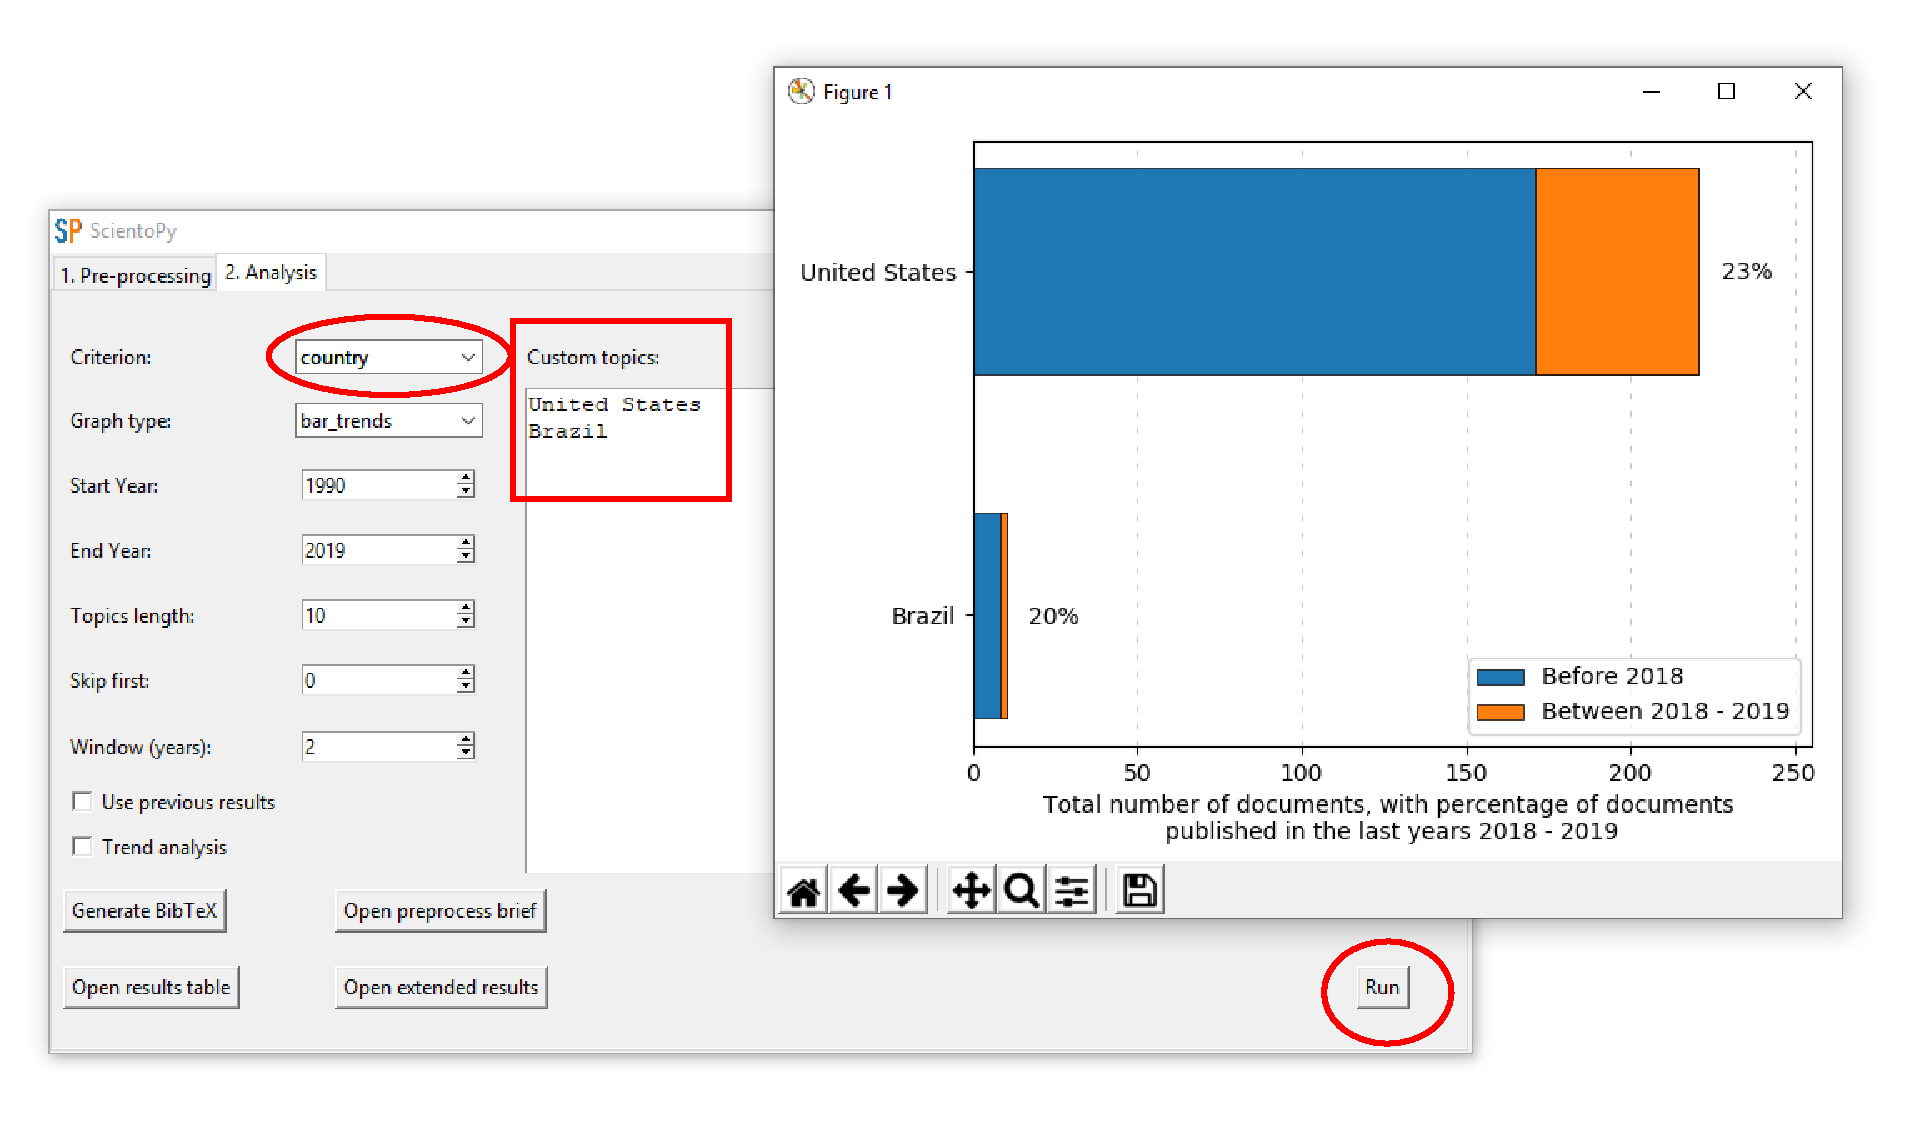
\includegraphics[width=0.8\textwidth]{./figures/win_analysis3.eps}
\end{center}

You can analyze any topic in any criterion. Also, you can integrate two or more topics in one, by dividing it with \verb|,|. This is very useful for abbreviations and plural singulars, for example: 
\begin{verbatim}
WSN, Wireless sensor network, Wireless sensor networks
RFID, RADIO FREQUENCY IDENTIFICATION
\end{verbatim}


\subsection{Asterisk (*) wildcard}

You can use the asterisk wildcard to find phrases or words which starts or ends with the letters that you have inserted. For example, if you want to find "device", "devices", and "device integration", entering \verb|device*| in the \verb|Custom topics| text box: 

\begin{center}
	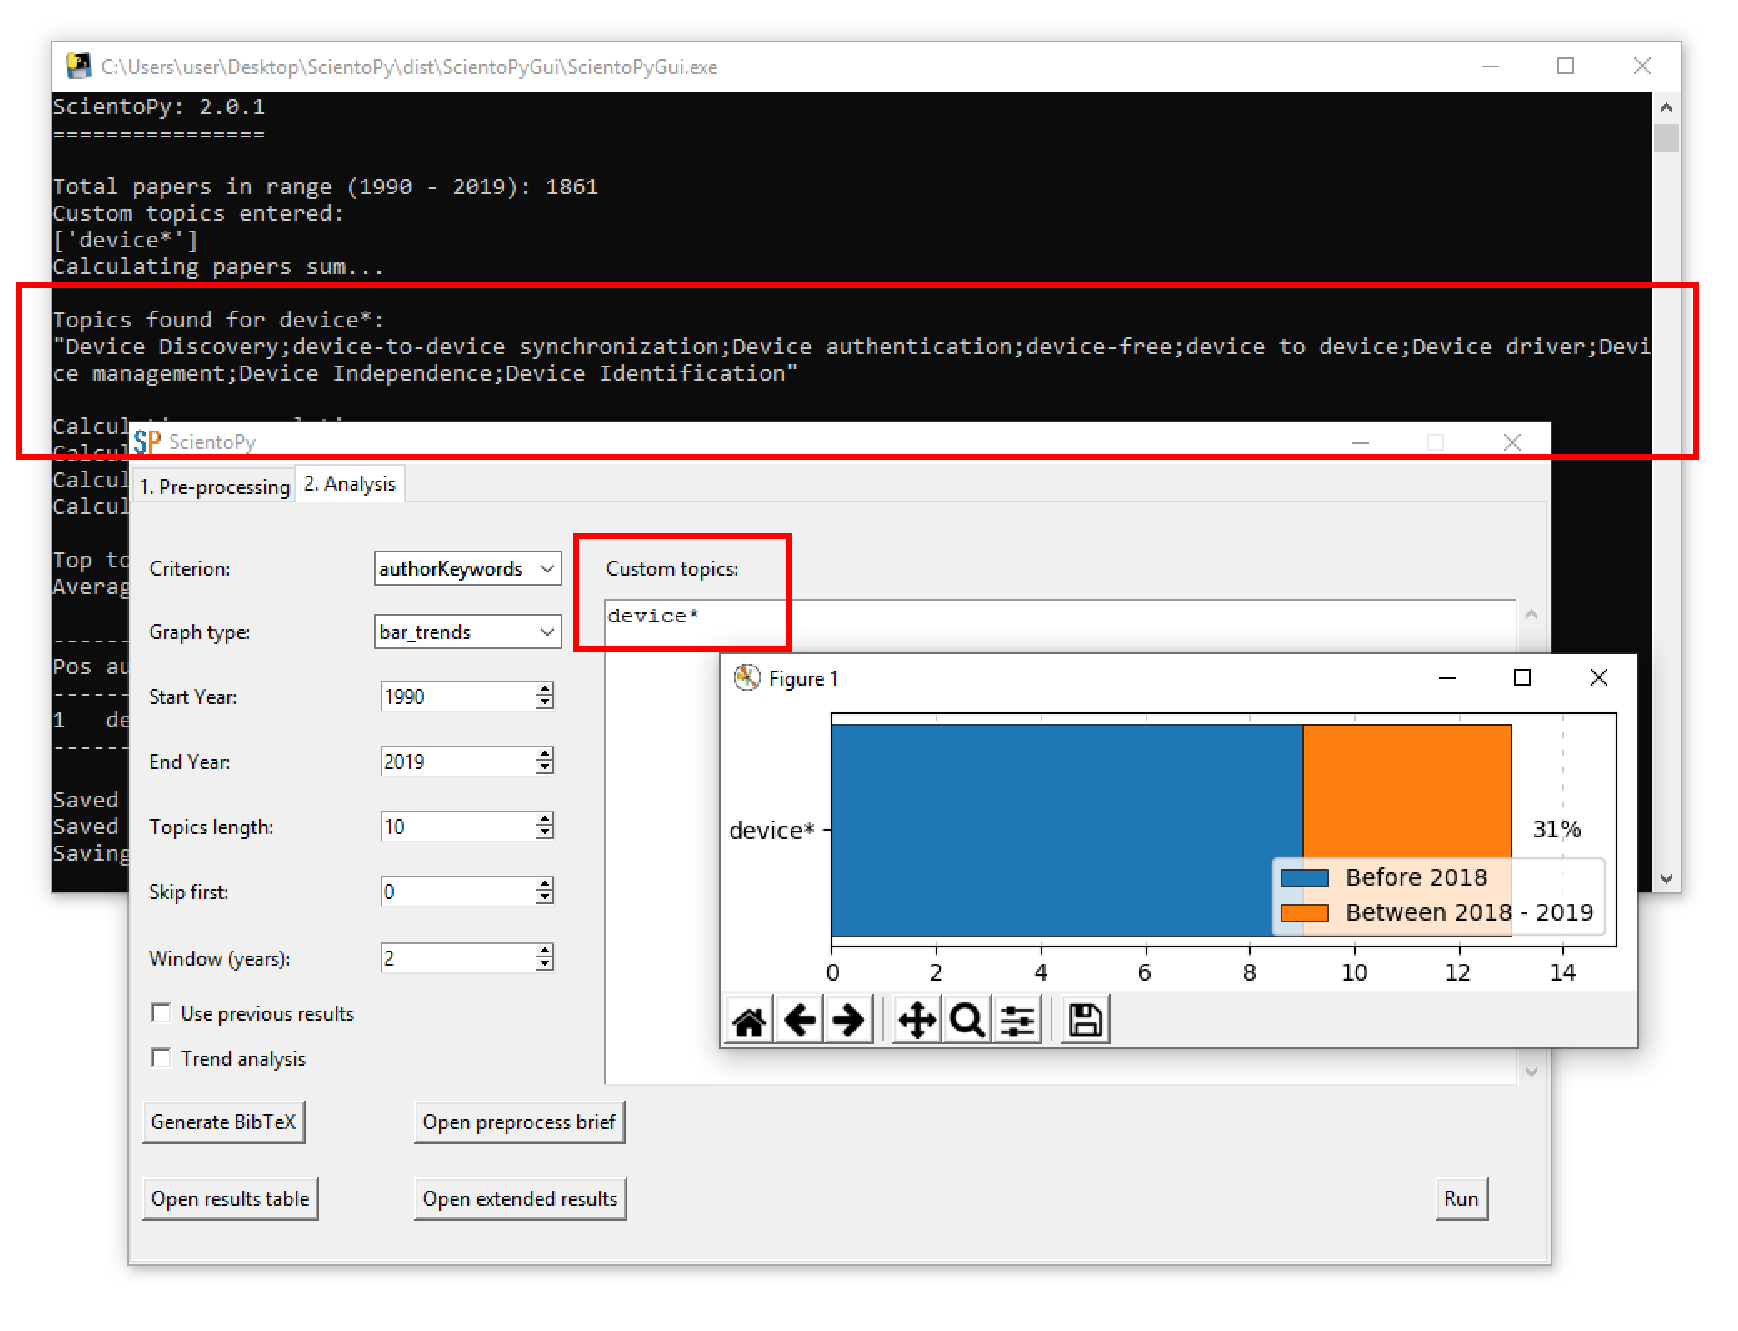
\includegraphics[width=0.8\textwidth]{./figures/win_analysis4.eps}
\end{center}

As shows in the firs red square, ScientoPy prints the topics found for the wildcard based search. You can copy this information, to analyze each specific topic found, like this (note, the \verb|;| is also used for topics separation): 
\begin{center}
	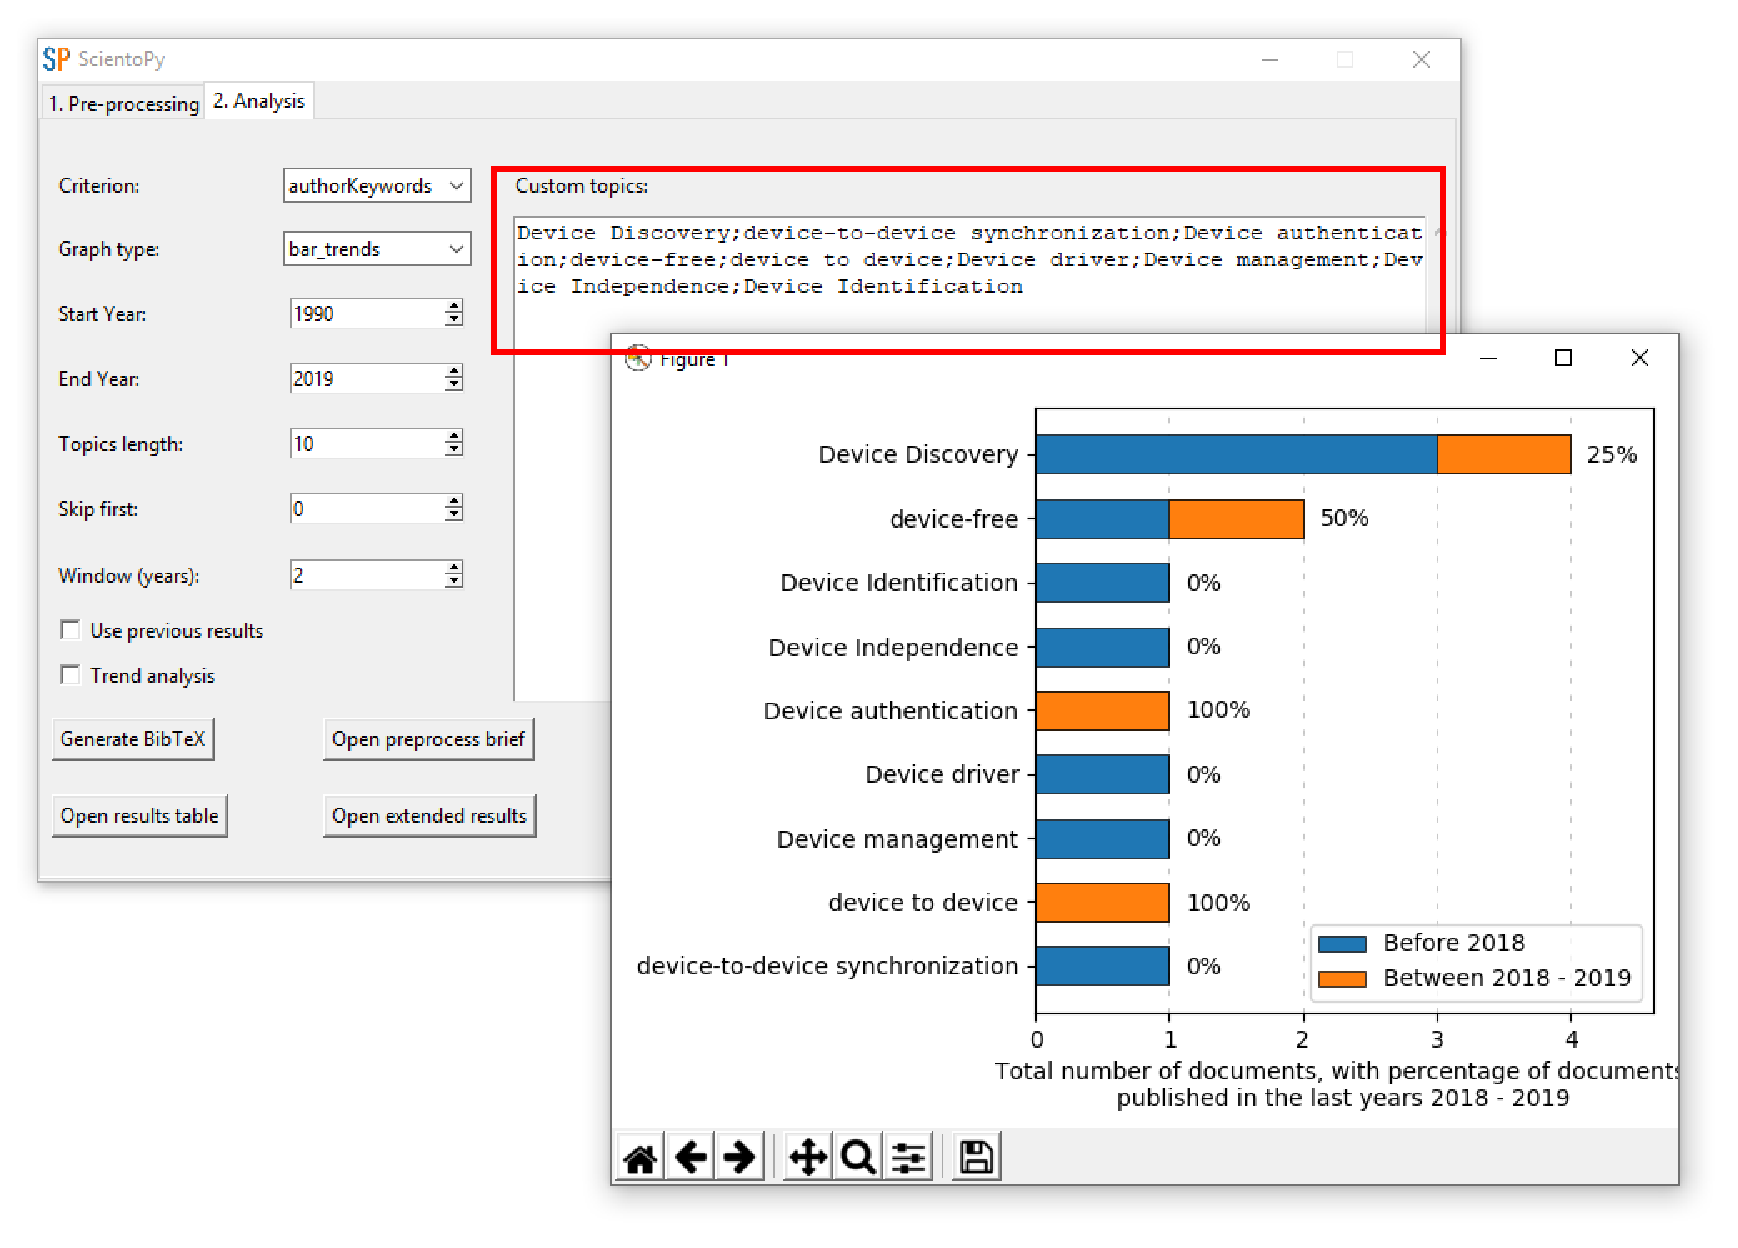
\includegraphics[width=0.8\textwidth]{./figures/win_analysis5.eps}
\end{center}

\subsection{Evolution plot}

Also, you can see the results with an evolution plot. This option plots the accumulative documents, average documents per year (ADY), and percentage of documents in the last years, for example:

\begin{center}
	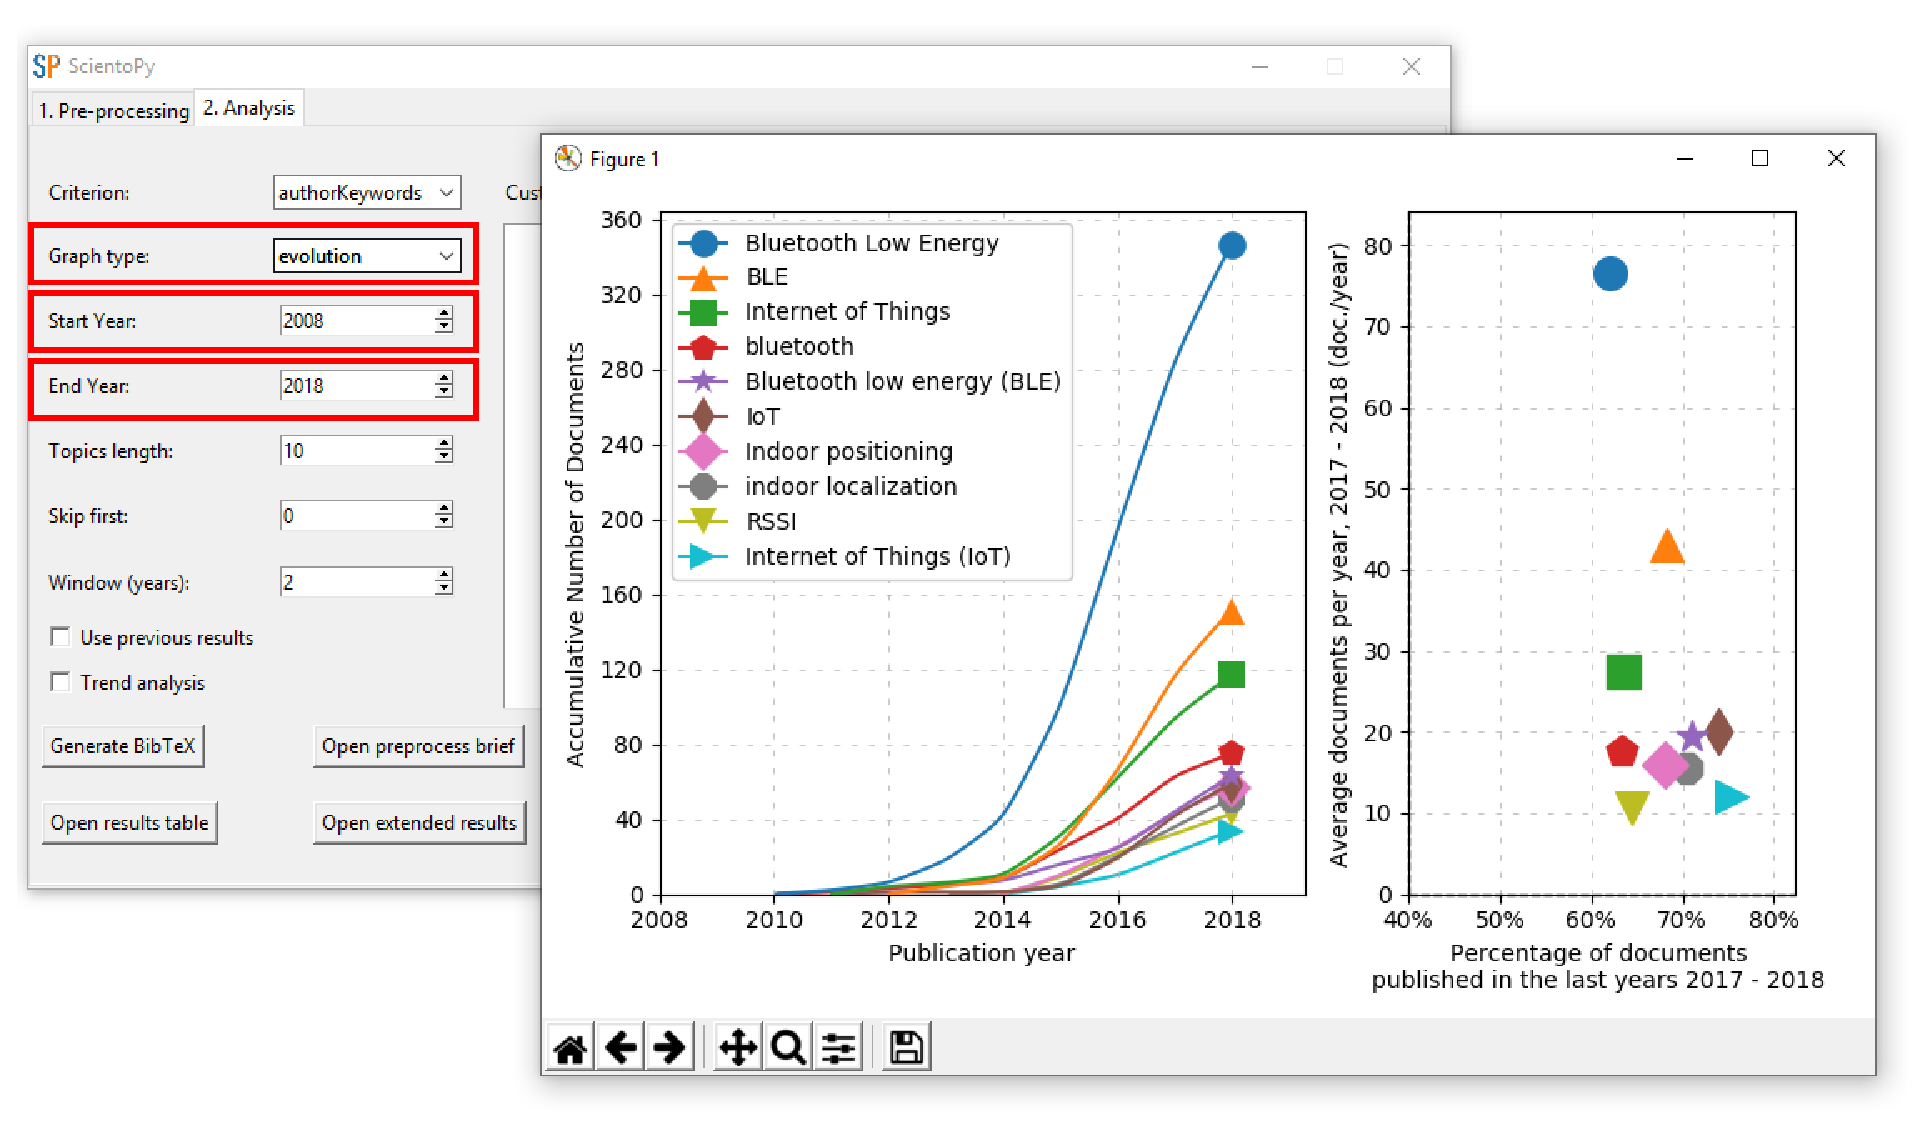
\includegraphics[width=0.8\textwidth]{./figures/win_analysis6.eps}
\end{center}

\textbf{Note:} select the right start and end years limit that fits better your plot lines.

\subsection{Finding trending topics}

This script finds the top trending topics based on the higher average growth rate (AGR) over the others. The AGR is calculated on two years periods, using the following Equation \eqref{equation_AGR}:
\begin{equation*}
AGR = \frac{\sum\limits_{i = Y_s}^{Y_e}P_i - P_{i-1}}{(Y_e - Y_s)+1},  
\label{equation_AGR}
\end{equation*}

\setlength{\leftskip}{5cm}
\hspace*{-1cm}where:\\
$AGR$ = Average growth rate;\\
$Y_s$ = Start year;\\
$Y_e$ = End year;\\
$P_i$ = Number of publications on year $i.$\\

\setlength{\leftskip}{0pt}

To find the top trending topics on author keywords criterion, you can run the following configuration: 

\begin{center}
	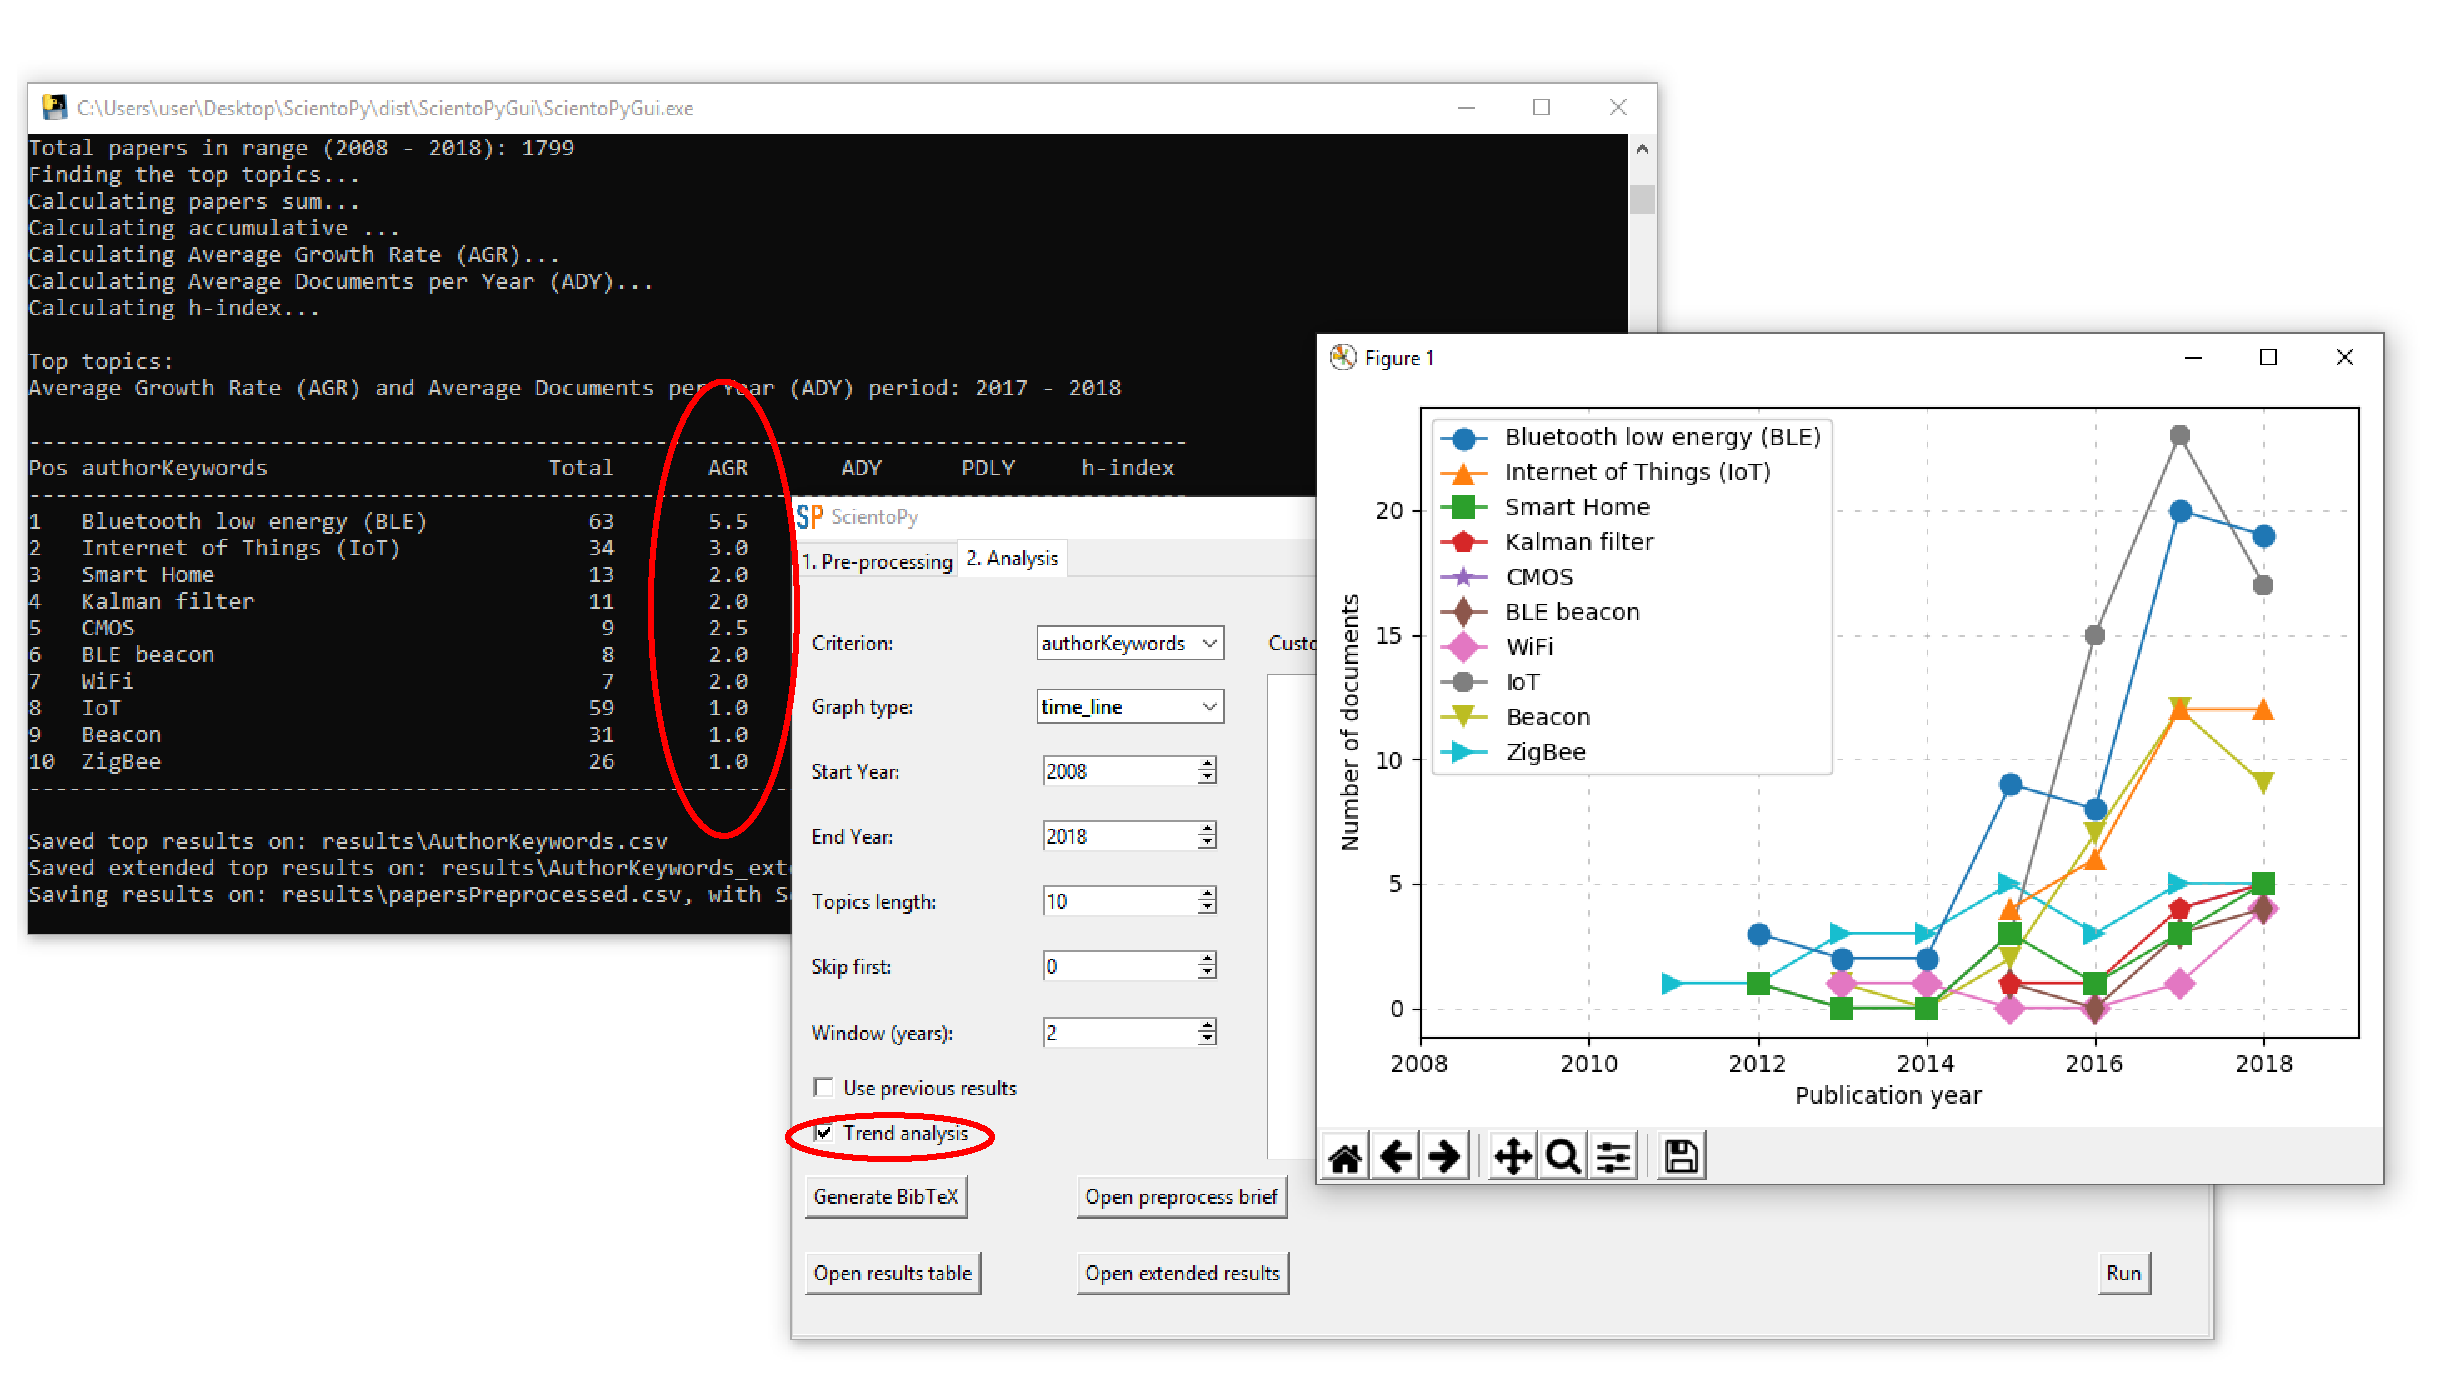
\includegraphics[width=0.8\textwidth]{./figures/win_analysis7.eps}
\end{center}

This script will find the top 200 topics, then it calculates the AGR for the last 2 years (\textit{Window (years): 2}). Finally, the 200 top topics are sorted from the highest AGR in the last 2 year period to the lower. 

\subsection{Analysis based on the previous results}

ScientoPy generates an output file with all the output documents from the last run script. For example if we run the following configuration:

\begin{center}
	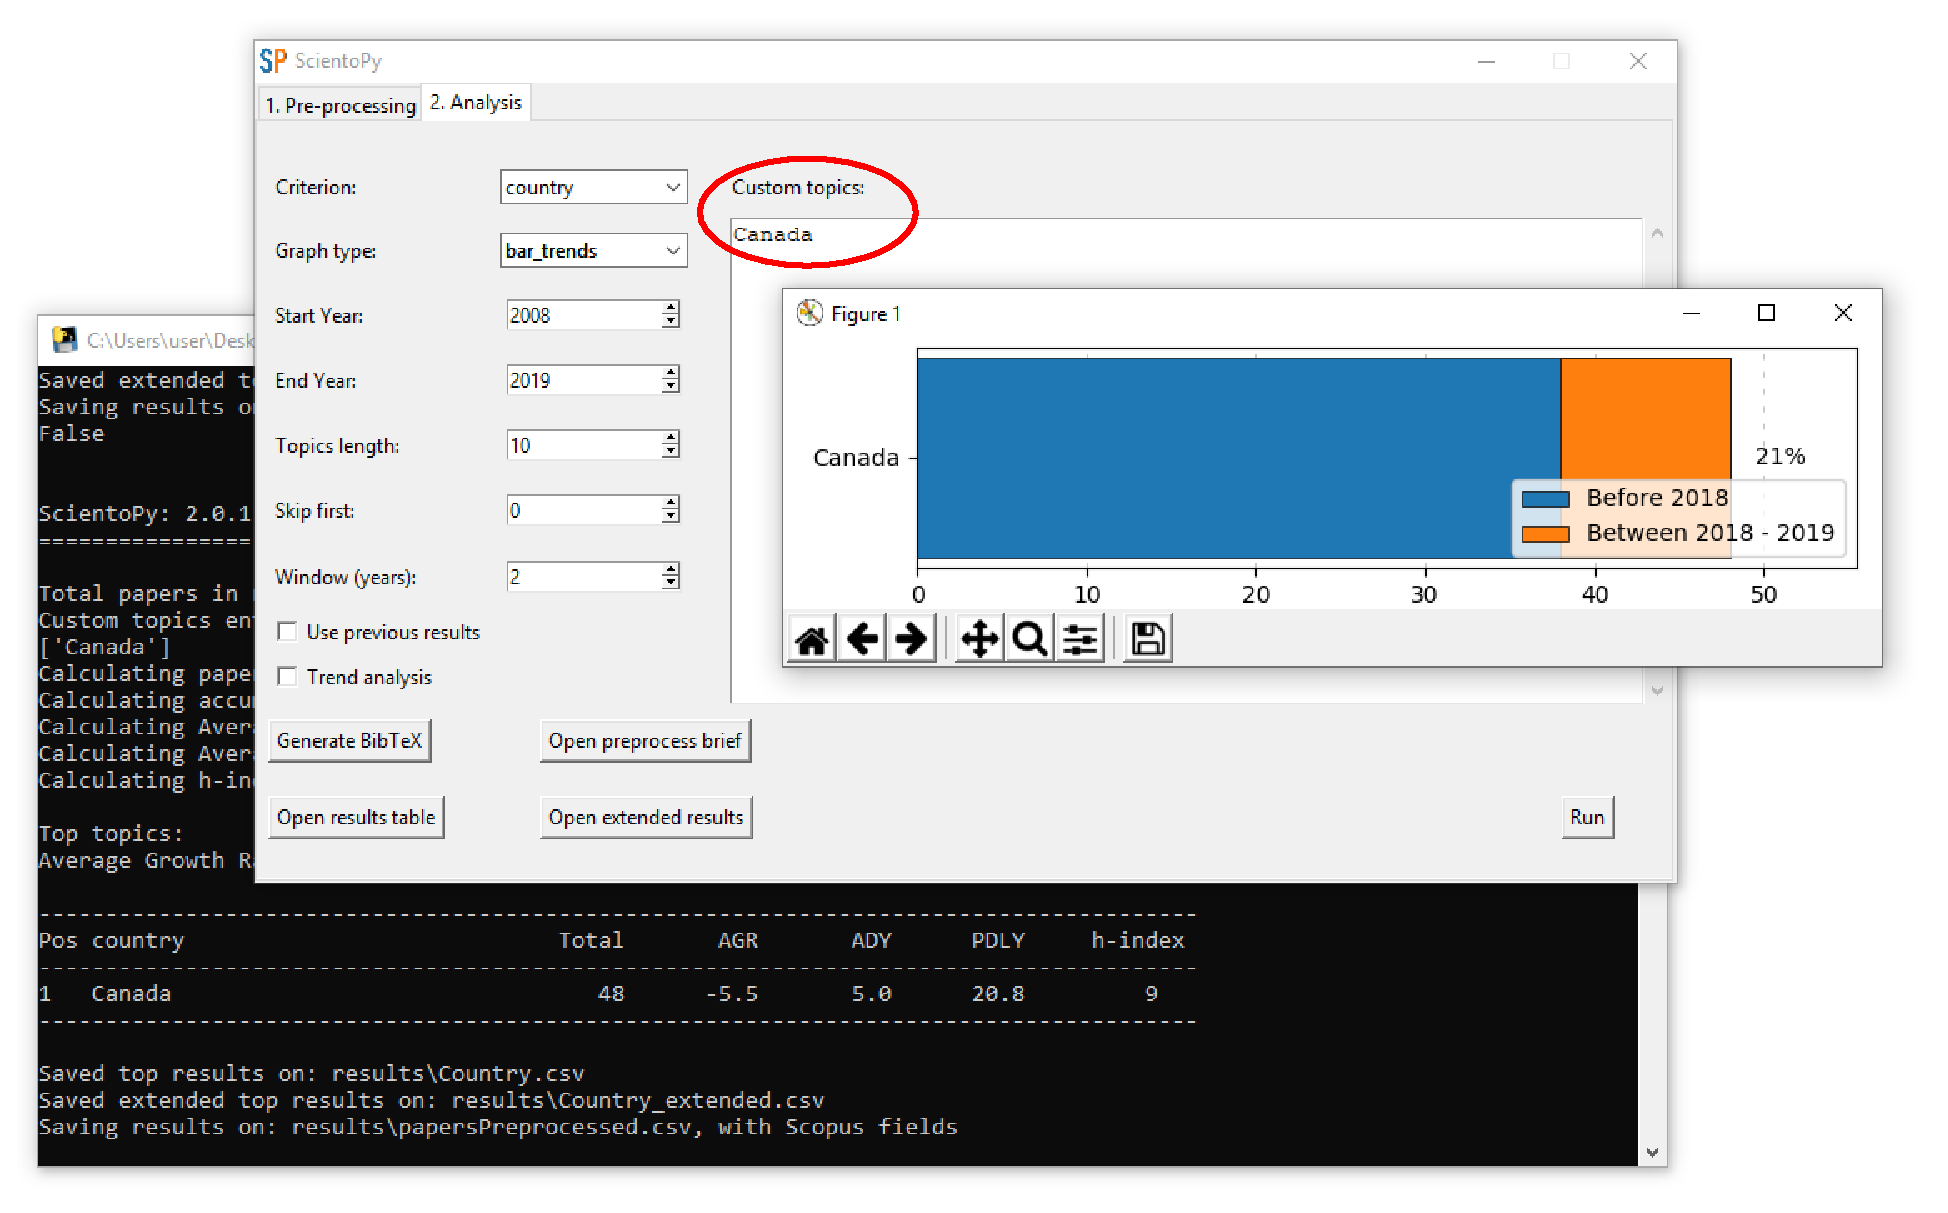
\includegraphics[width=0.8\textwidth]{./figures/win_analysis8.eps}
\end{center}

ScientoPy will create a documents output file (\verb|results/papersPreprocessed.tsv|) with all documents that have authors with affiliation in Canada. This output file can be used by ScientoPy to perform an analysis based on this, in that way if we check the option \verb|Use previous results|, and we select in \verb|Criterion| authorKeywords we will obtain the top author keywords from papers where the author affiliation correspond to Canada. Also, we can run the following configuration to know which are the countries that have more common documents with Canada:

\begin{center}
	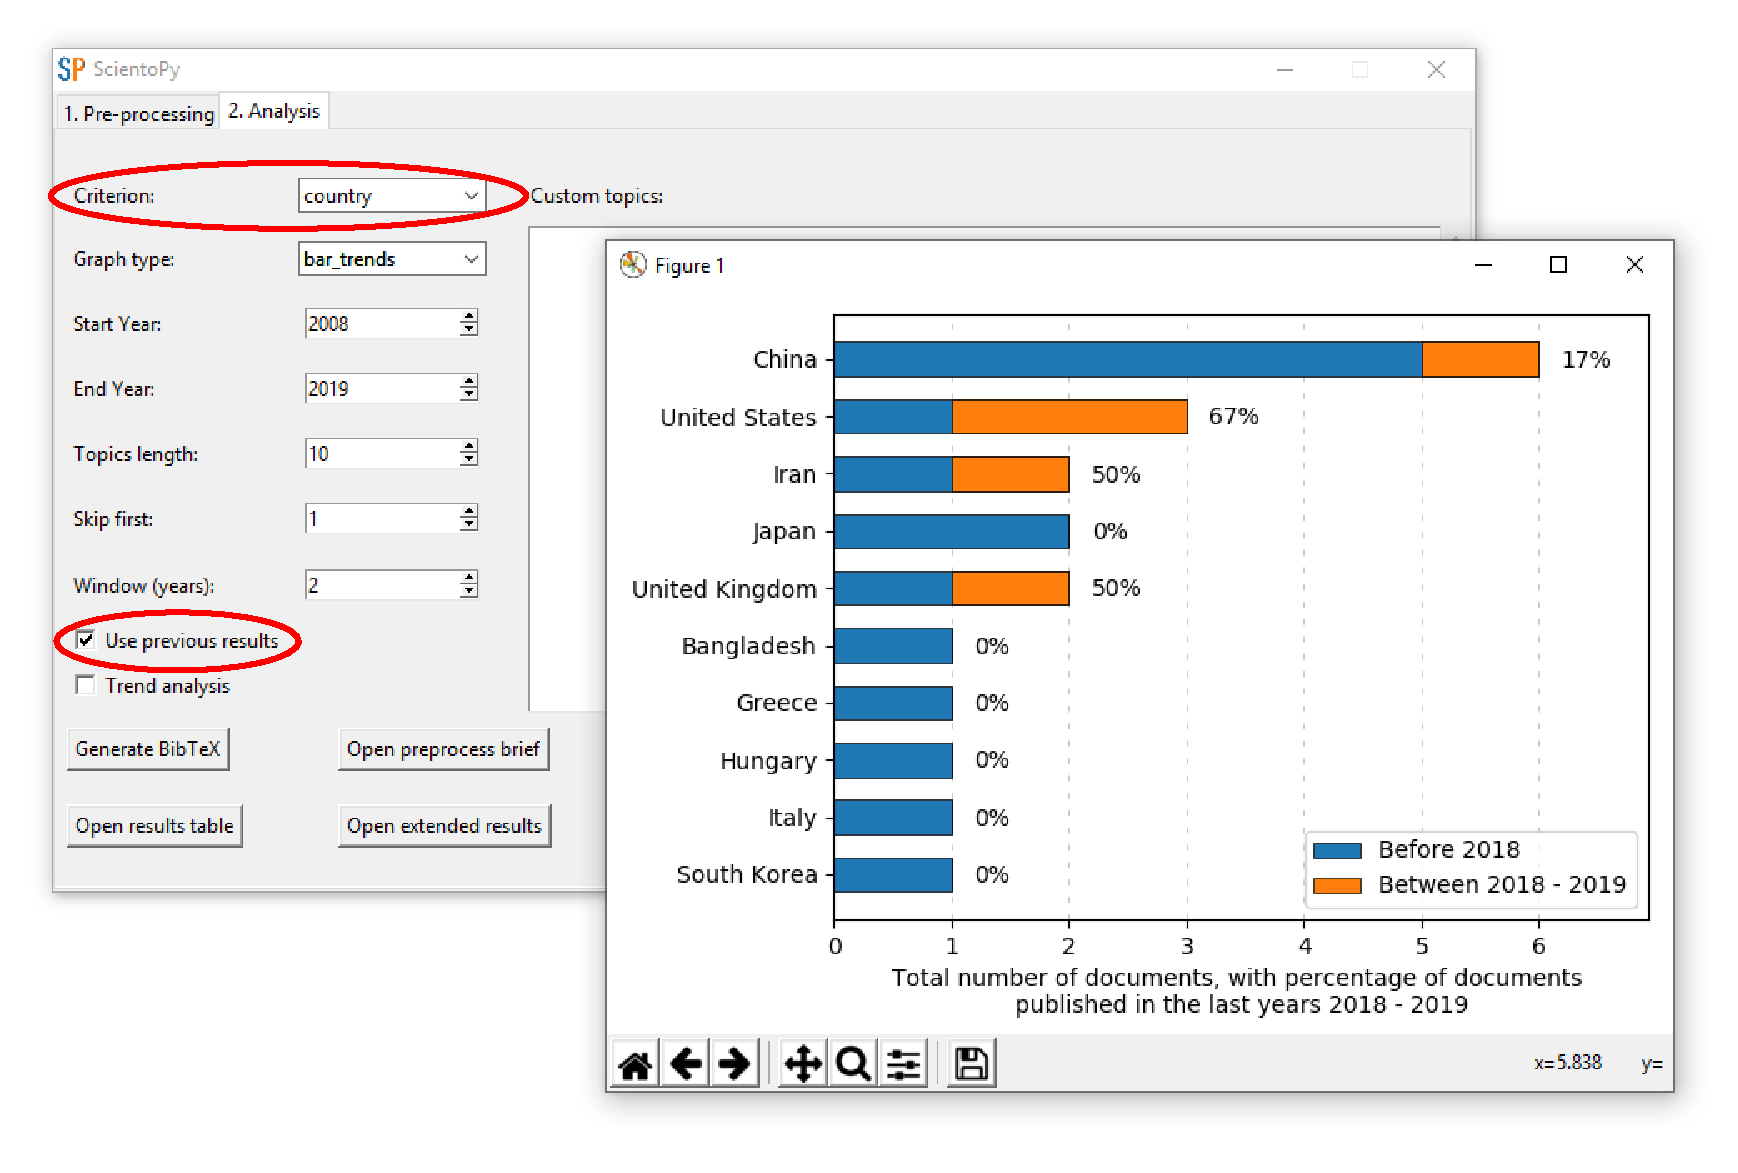
\includegraphics[width=0.8\textwidth]{./figures/win_analysis9.eps}
\end{center}

\textbf{Note:} the ScientoPy documents output file is only generated when the \verb|Use previous results| is not marked. In that way, if we run many times a ScientoPy command with this option, the documents output file will not overwritten.

\section{Generate BibTeX}

With ScientoPy you can generate a \LaTeX BibTeX file for your reference. For this follow the next steps:

\begin{enumerate}
\item Open the extended results from your analysis, by clicking the \verb|Open extended results| button.
\item Copy the EID value of the paper or papers that you want to cite to the latex document inside the \verb|\cite{}| preamble, as shown in the following figure:

\begin{center}
	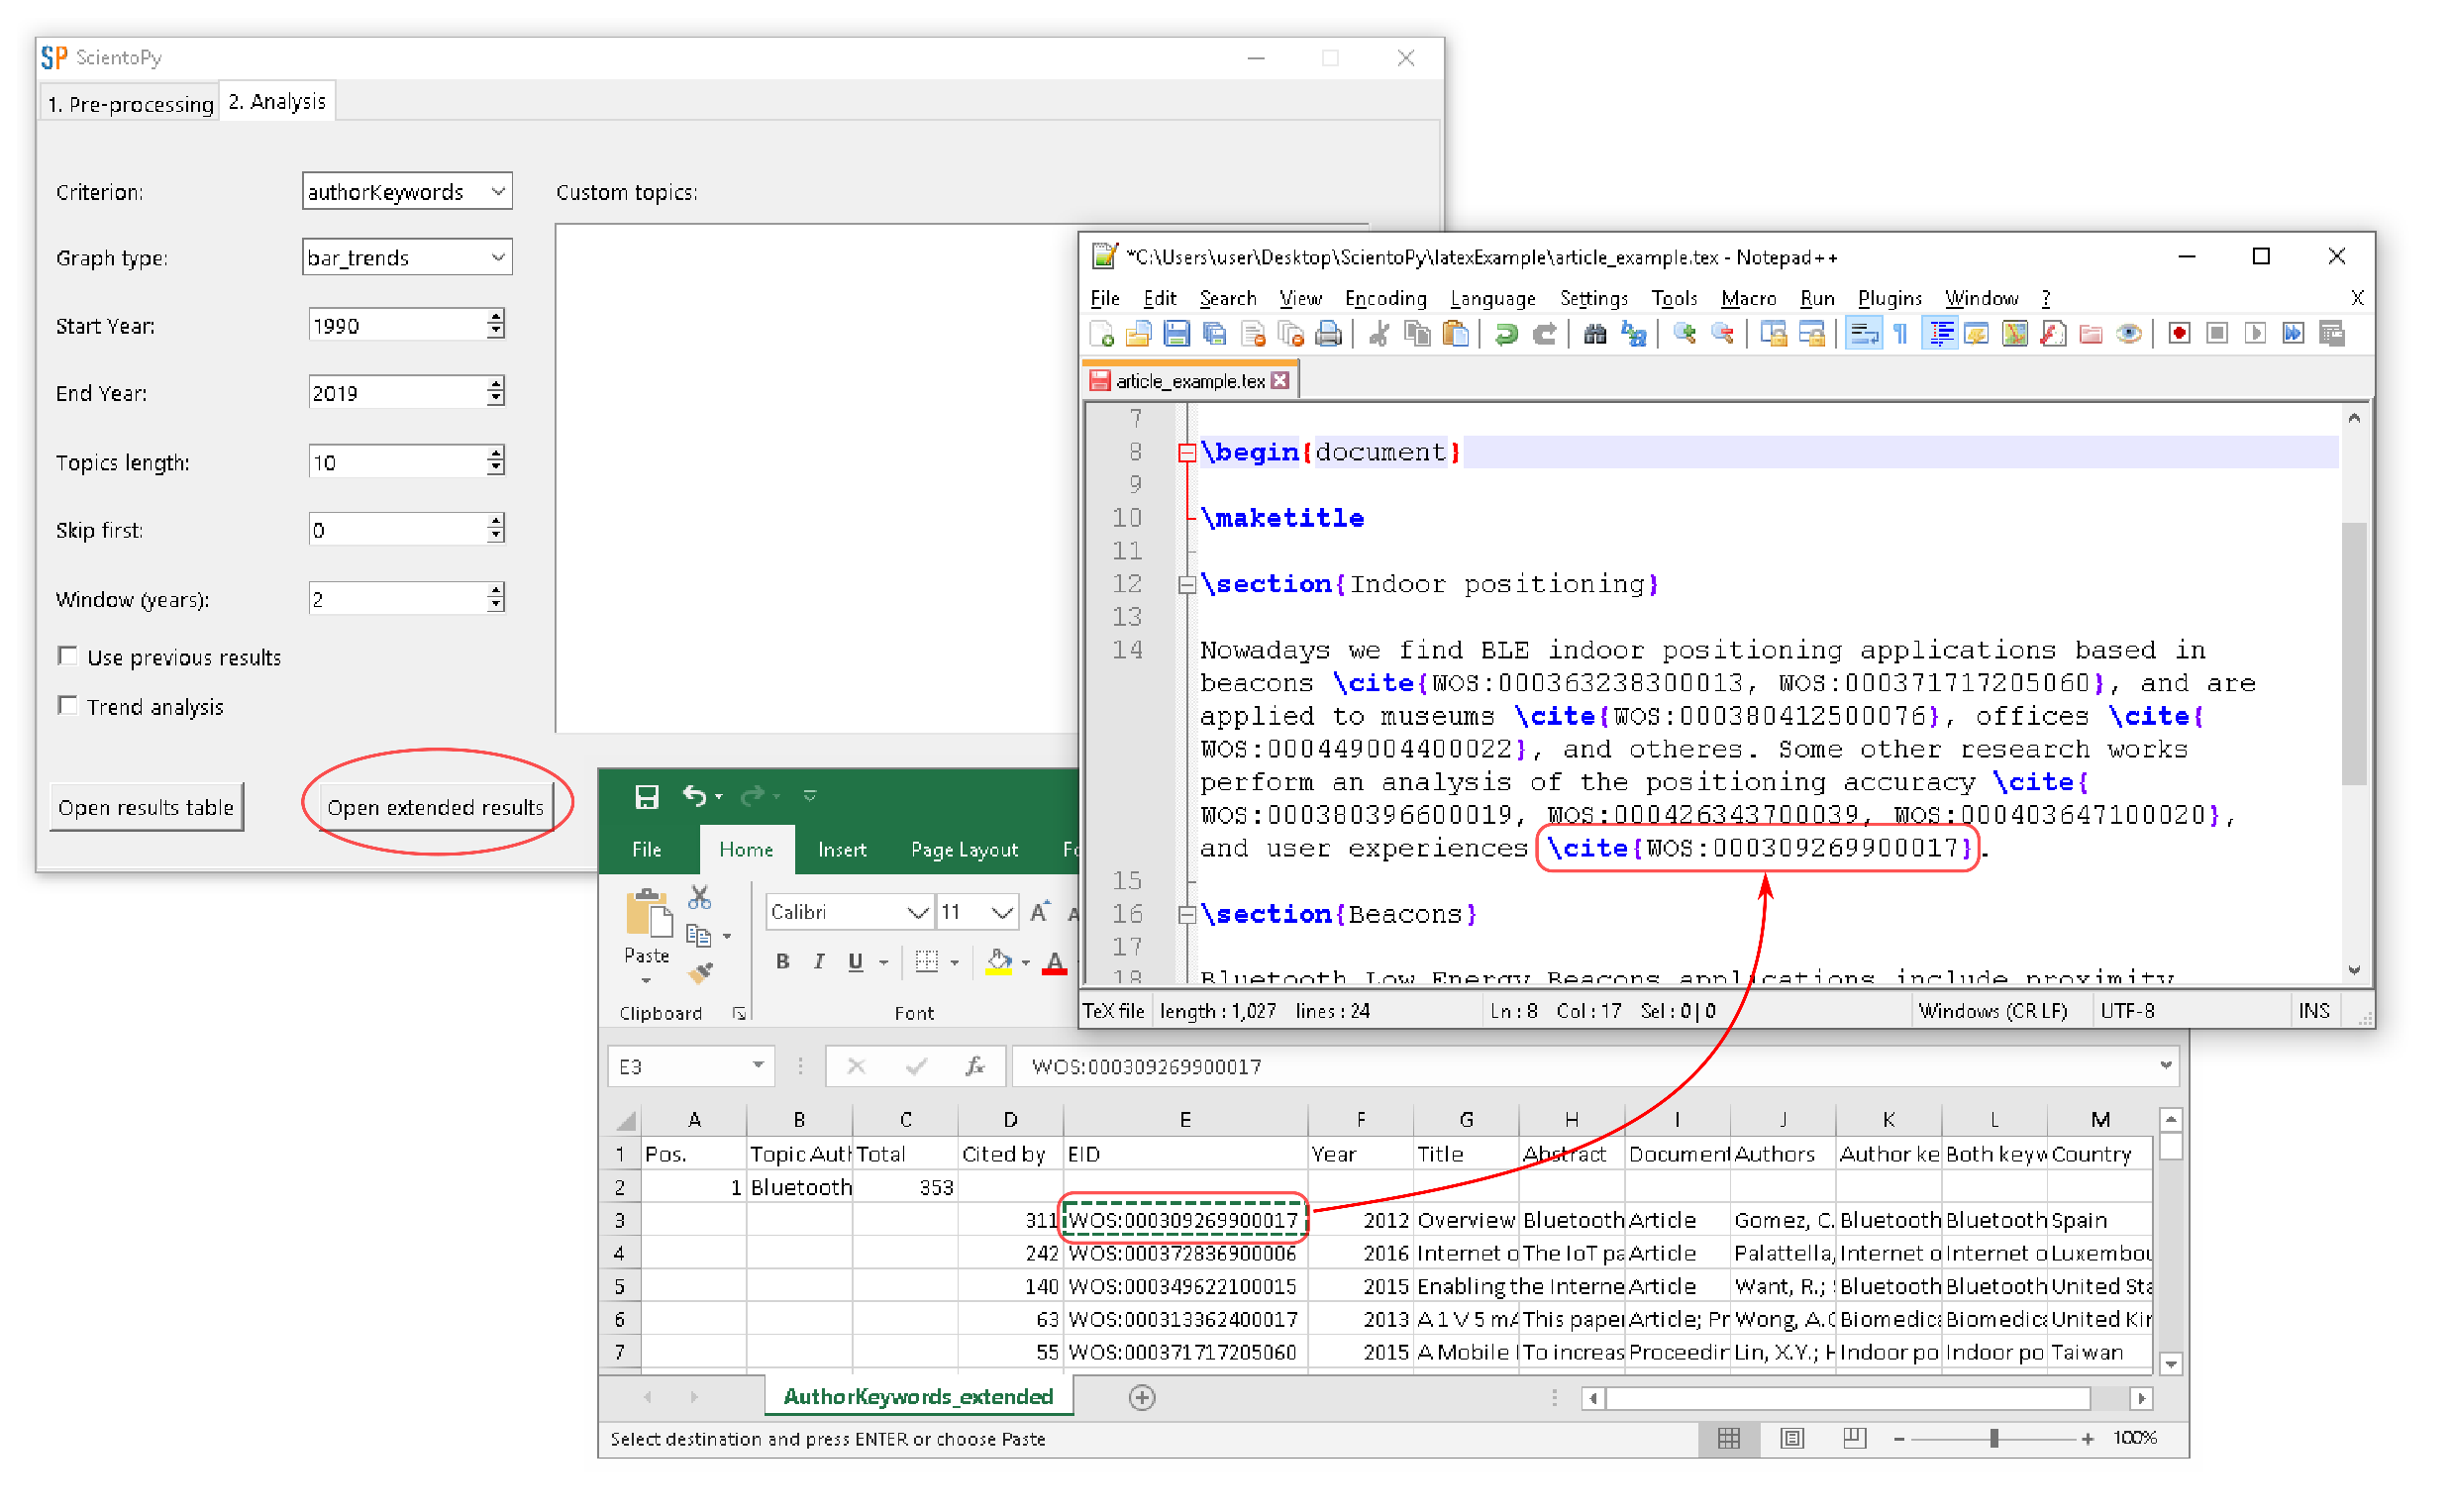
\includegraphics[width=0.9\textwidth]{./figures/win_generate_bib1.eps}
\end{center}

\item Save your LaTeX document 

\item Push the button \verb|Generate BibTeX| and select the LaTeX document where you have added the EID

\item ScientoPy will look for all EID in the document and will generate the BibTeX information from the dataset preprocessed. Finally it will open the BibTeX file in a text editor in order, as shown in the following figure:

\begin{center}
	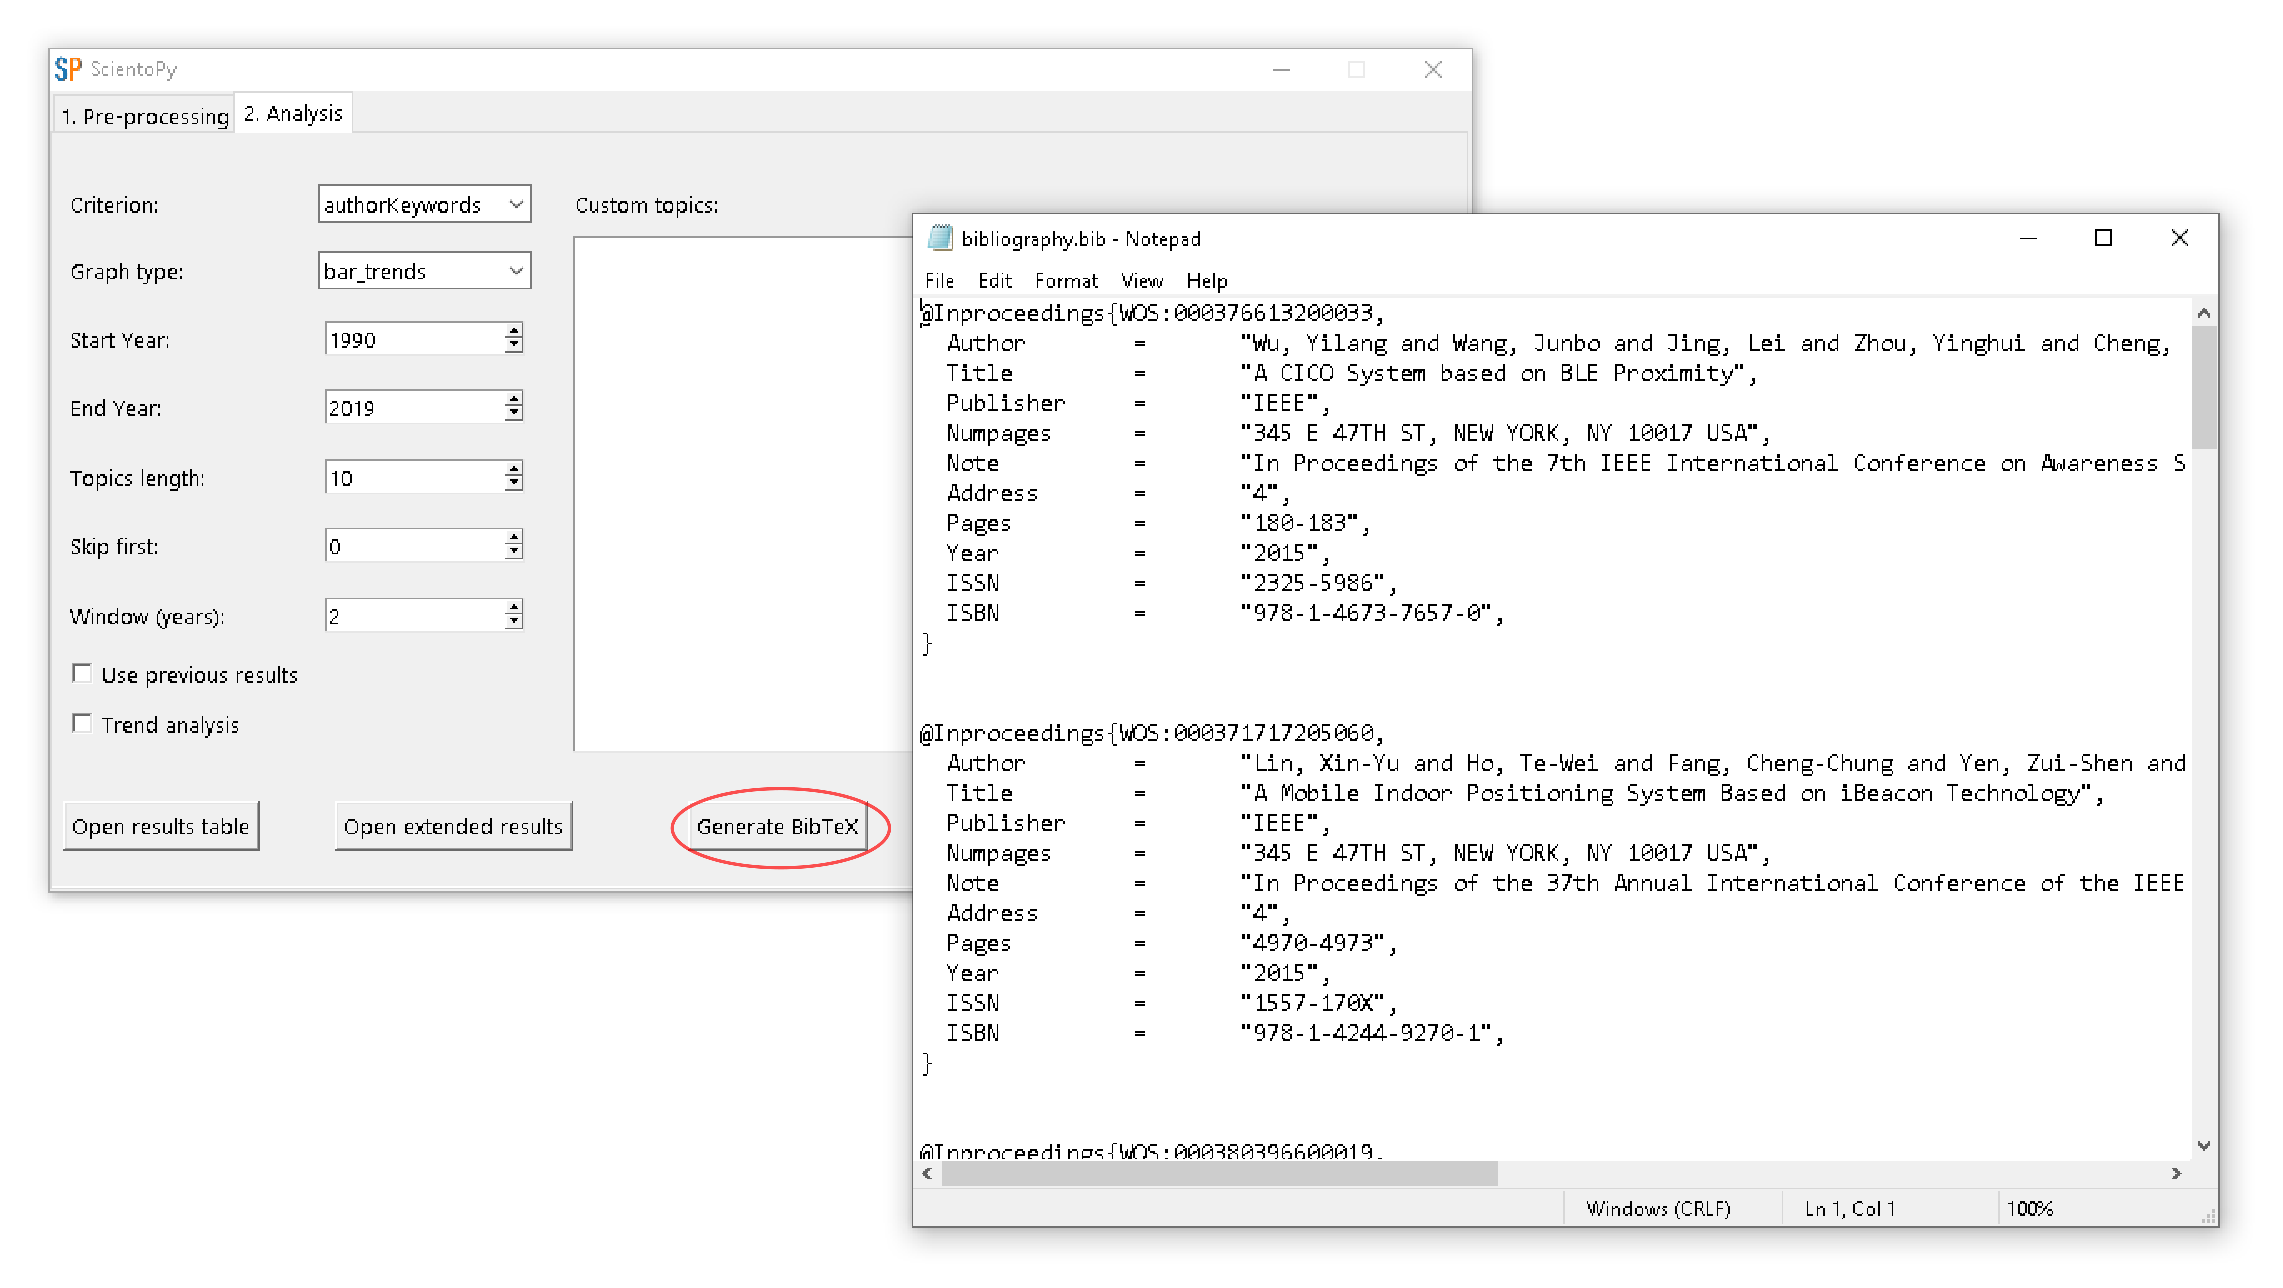
\includegraphics[width=0.8\textwidth]{./figures/win_generate_bib2.eps}
\end{center}

\end{enumerate}

\textbf{Note:} for your reference we have included an article LaTeX file example in the location \verb|latexExample/article_example.tex|. This have cites from the example dataset. To test the Generate BibTeX capability, you can follow the next steps:
\begin{itemize}
\item Preprocess the example dataset located in \verb|dataInExample|, 
\item Click in \verb|Generate BibTeX| 
\item Select the file \verb|latexExample/article_example.tex| 
\item Save the generated \verb|bibliography.bib| file in the \verb|latexExample| folder 
\item Compile the \verb|latexExample/article_example.tex| file, with the command \verb|latexmk -pdf article_example.tex|
\end{itemize}

\section{Output files and directories}

After run ScientoPy analysisyou will find the following folder and files structure:

\vspace*{0.5cm}
\dirtree{% This % is required
	.1 ScientoPy.
	.2 dataInExample.
	.2 dataPre.
	.3 papersPreprocessed.tsv.
	.3 PreprocessedBrief.tsv.
	.2 graphs.
	.2 latexExample.
	.2 Manual.
	.2 results.
	.3 AuthorKeywords.tsv.
	.3 AuthorKeywords\_extended.tsv.
	.3 papersPreprocessed.tsv.
}

These folders and output files are described bellow:

\begin{itemize}
	\item \textbf{dataInExample: } contains Scopus and WoS example data set for the search criteria "Internet of things" AND "Gateway" downloaded in 27 November 2017. This is the input example for preprocess script.
	
	\item \textbf{dataPre: } output folder for the preprocess results, and input folder for scientoPy script.
	
	\item \textbf{papersPreprocessed.tsv: } preprocesed papers data with all input documents merged, filtered, and duplication removed. This is the input file that scientoPy script uses.
	
	\item \textbf{PreprocessedBrief.tsv: } preproceses brief table that shows the preprocess results related to total papers found per data base, the omitted papers, the duplicated papers count per data base, and the total number of papers per paper type (Conference paper, article, review...)
	
	\item \textbf{graphs: } graphs output folder for preprocess and scientoPy scripts

	\item \textbf{latexExample: } folder with the LaTeX file article example to generate the BibTeX from the preprocess dataset. 

	\item \textbf{Manual: } folder with the pdf manual and example paper with scientoPy commands highlighted used for graph and tables generation. 
	
	\item \textbf{results: } output folder for scientoPy result output files
	
	\item \textbf{AuthorKeywords.tsv: } scientoPy output file for the selected criterion (in this case authorKeywords) that shows the top topics or the custom  topics with the total number of documents, the Average Growth Rate (AGR), the Average Documents per Year (ADY), the h-index, and the documents per each year. 
	
	\item \textbf{AuthorKeywords\_extended.tsv: } scientoPy output file for the selected criterion (in this case authorKeywords) that show the top or custom topics with the documents related to each one.
	
	\item \textbf{papersPreprocessed.tsv: } inside the results folder, this file contains the output papers from the last scientoPy used script. This is used as an input for scientoPy script when we mark the option \verb|Use previous results|.
\end{itemize}

\newpage
\section{ScientoPy graph types}

ScientoPy has 5 different ways to graph the results described on Table \ref{table_graph_types}.

\begin{table}[!h]
	\centering
	\caption{ScientoPy output graphs types}
	\label{table_graph_types}

	\renewcommand{\arraystretch}{1.5}
	\begin{tabular}{ p{4cm} p{3cm} p{10cm}}
	\hline\noalign{\smallskip}
	Graph type     &  Abreviation & Description                             \\
	\noalign{\smallskip}\hline\noalign{\smallskip}                                                                         
	Time line      & \verb|time_line| & Graphs the number of documents of each topic vs the publication year \\
	Horizontal bars  & \verb|bar| & Graphs the total number of documents of each topic in horizontal bars \\
	Horizontal bars trends  & \verb|bar_trends| & Graphs the total number of documents of each topic in horizontal bars, with the percentage of document published in the last years \\
	Evolution     & \verb|evolution| & Graphs two plots, one with the accumulative number of documents vs the publication year, and other with the average papers per year vs the percentage of documents in the last years\\
	Word cloud     & \verb|word_cloud| & Generate a word cloud based on the topic total number of publications \\
	\noalign{\smallskip}\hline
	\end{tabular}
\end{table}

Below are showed some examples of these graphs types, with the command used.

\subsection{Time line graph}
\begin{center}
	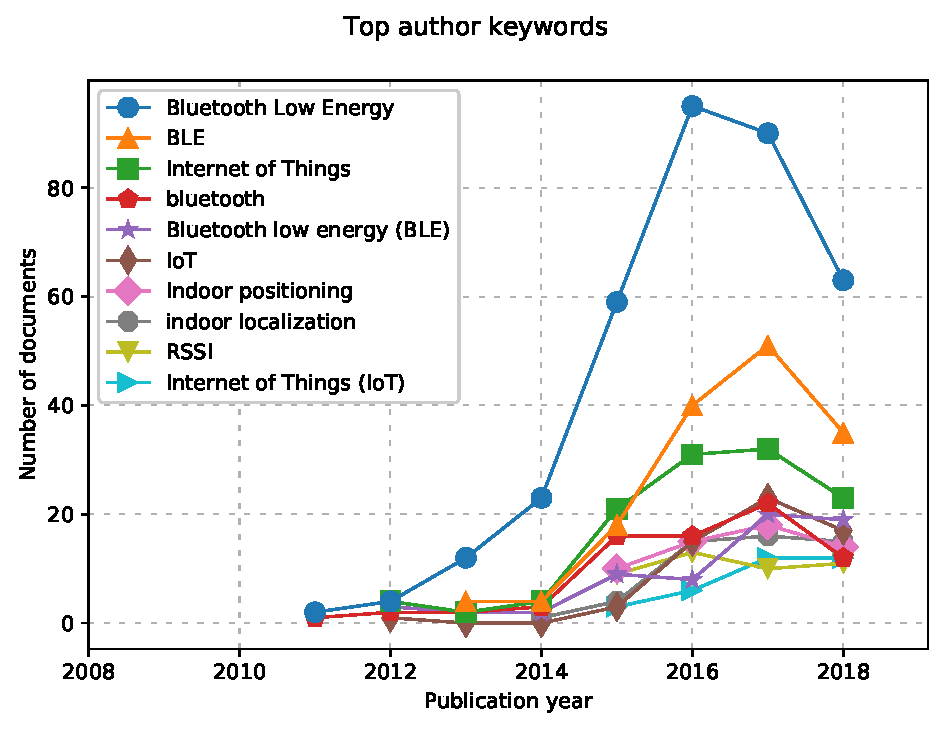
\includegraphics[width=0.75\textwidth]{./figures/graph_time_line.eps}
\end{center}

\subsection{Horizontal bars graph}
\begin{center}
	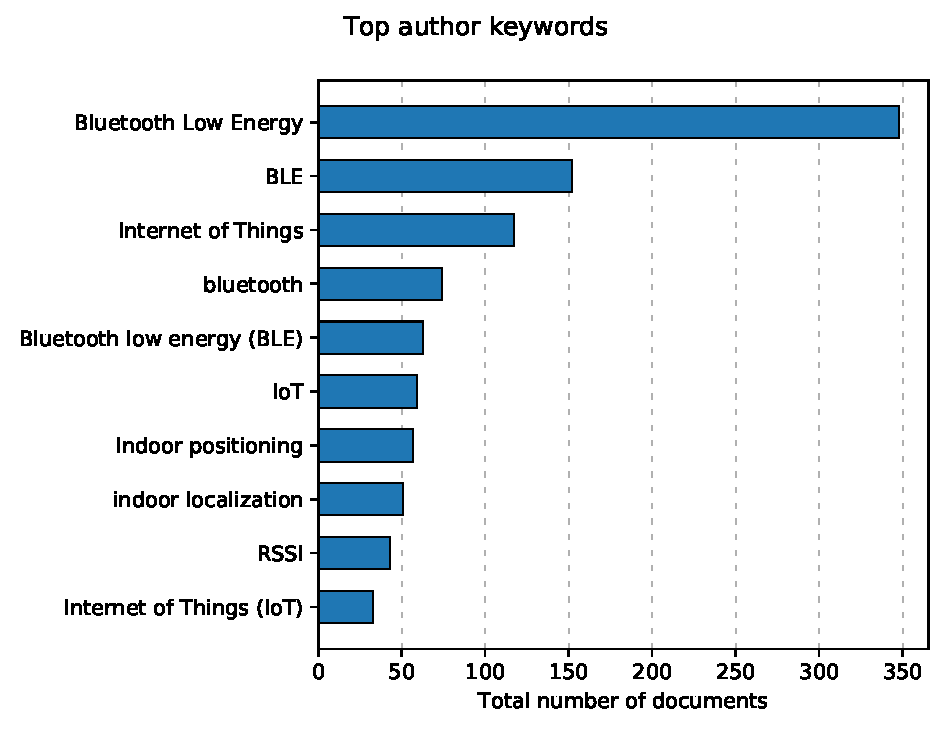
\includegraphics[width=0.75\textwidth]{./figures/graph_bar.eps}
\end{center}

\subsection{Horizontal bars trends}

\begin{center}
	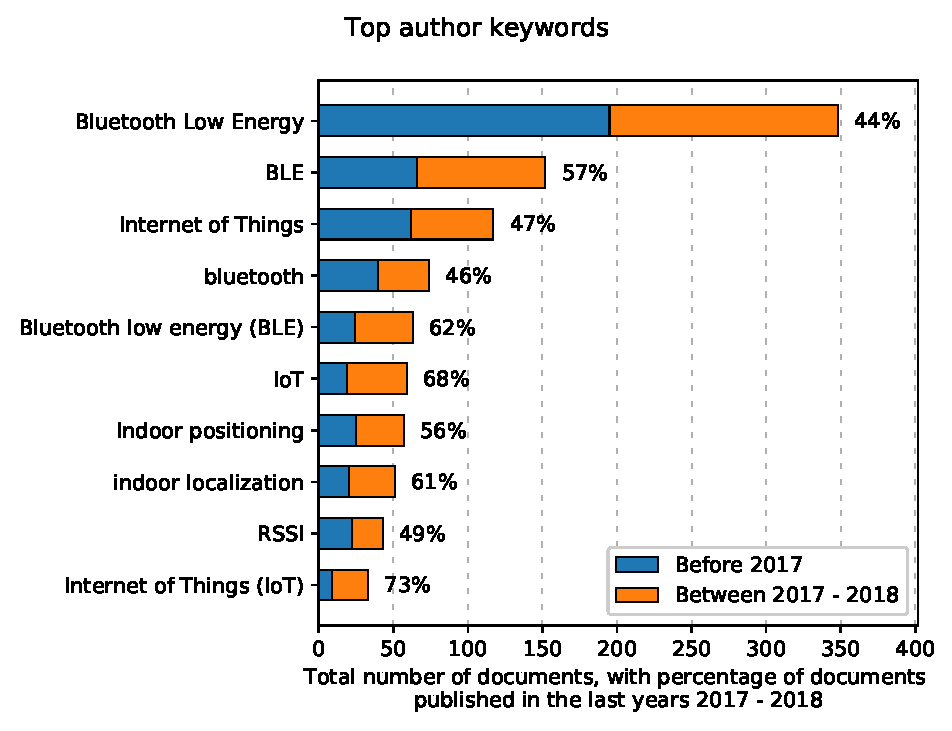
\includegraphics[width=0.75\textwidth]{./figures/graph_bar_trends.eps}
\end{center}

\subsection{Evolution graph}

\begin{center}
	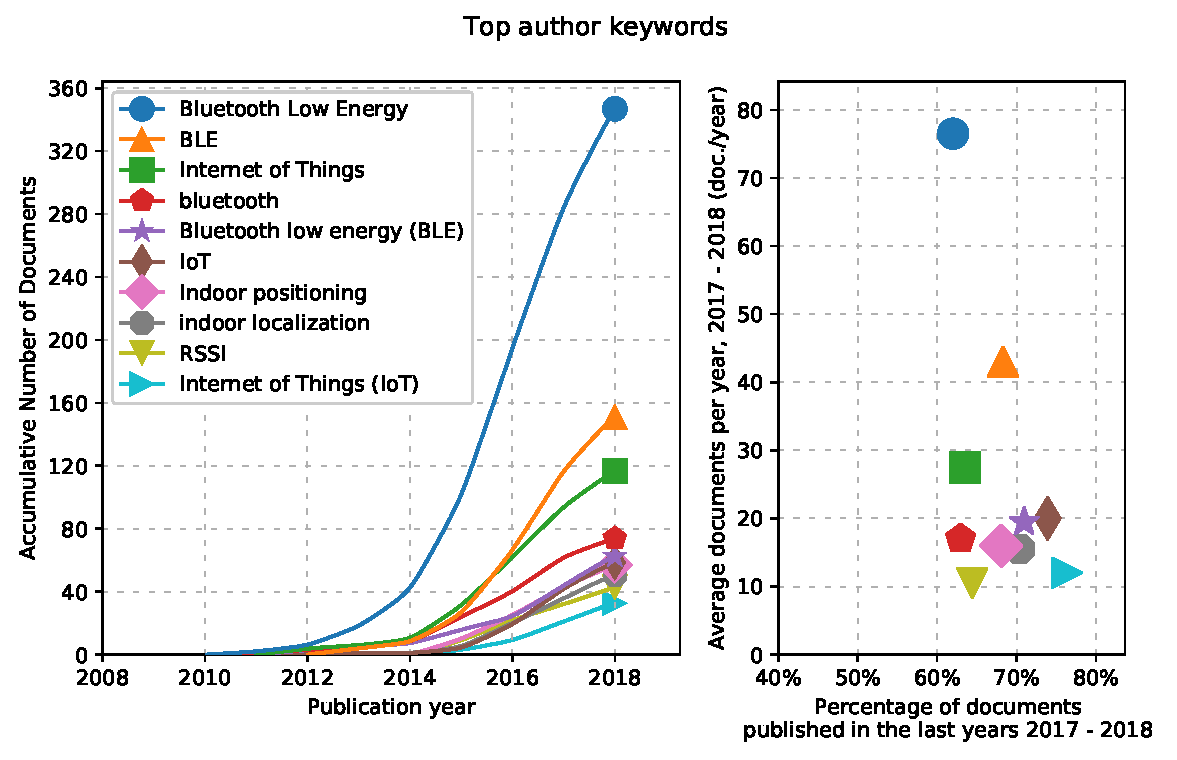
\includegraphics[width=0.75\textwidth]{./figures/graph_evolution.eps}
\end{center}


\subsection{Word cloud graph}

\begin{center}
	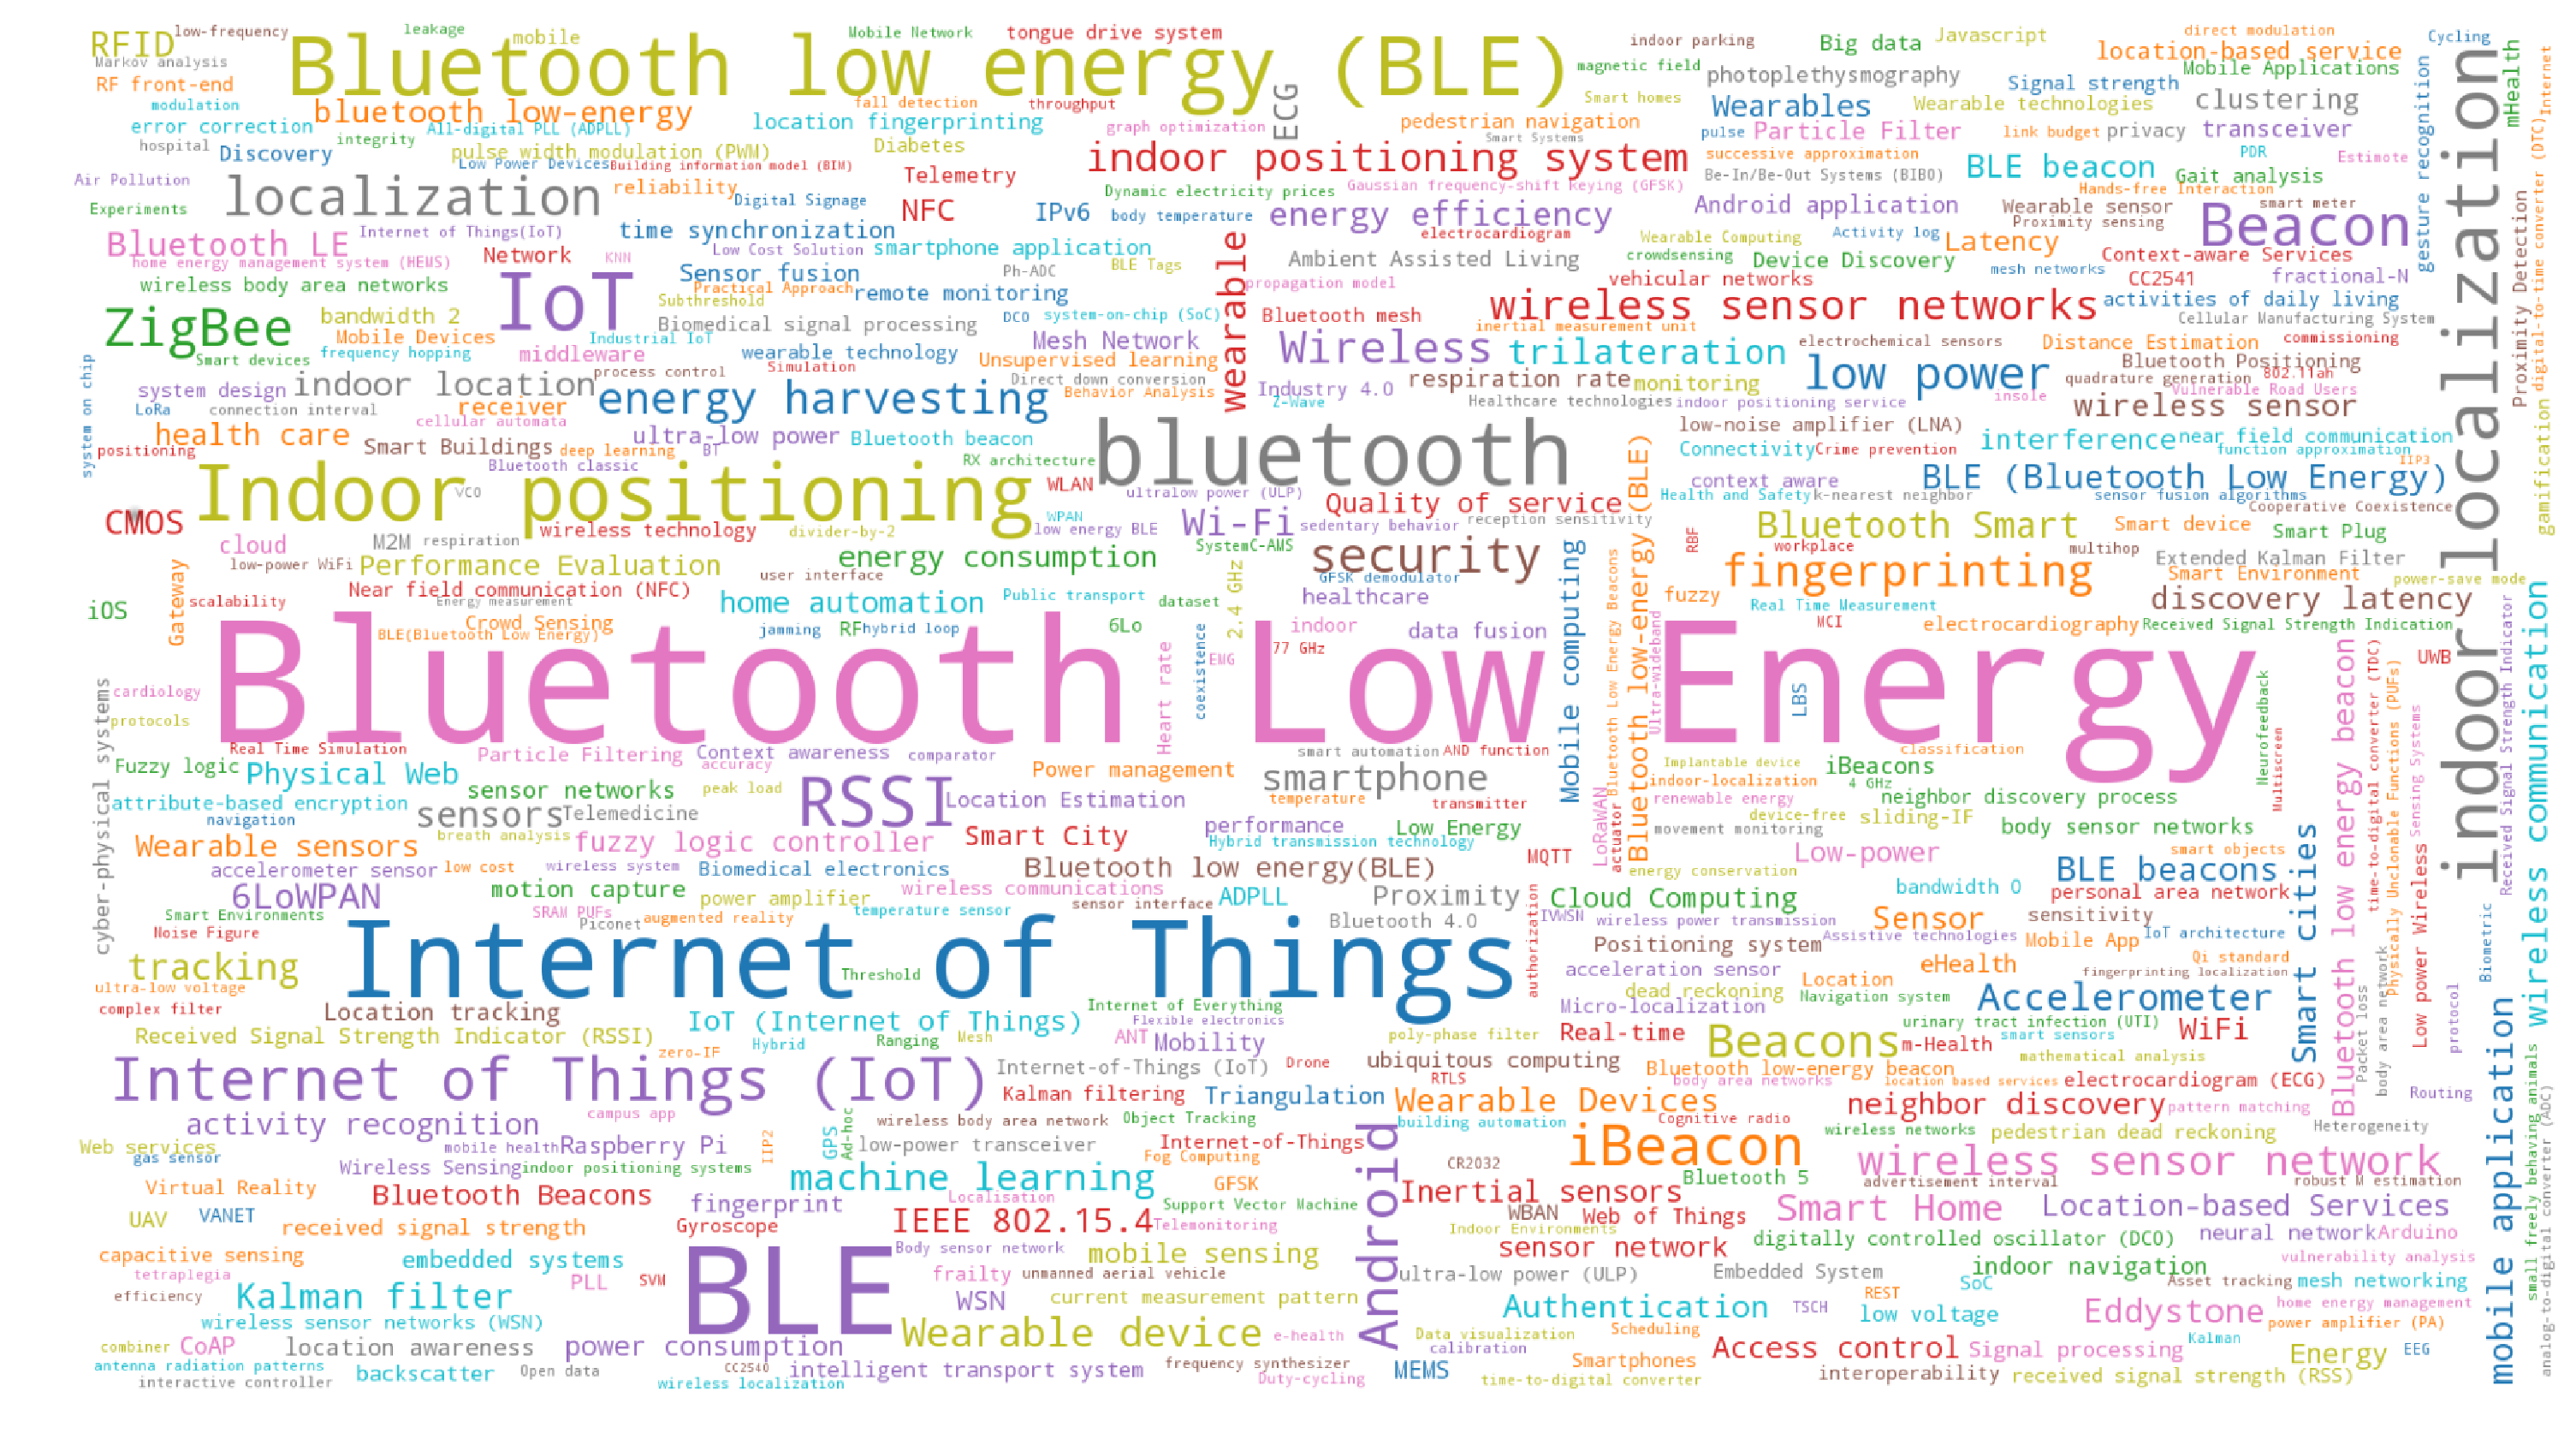
\includegraphics[width=0.9\textwidth]{./figures/graph_word_cloud.eps}
\end{center}


\end{document}  
